\documentclass[10pt,a4paper]{report}
\usepackage{mystyle}
\usepackage[margin=1.5in]{geometry}
\usepackage{amsmath}
\usepackage[toc,page]{appendix}
\graphicspath{{../../}} % results/ will reference results.

%%% Multiple Appendicies
\makeatletter
  \@addtoreset{chapter}{part}
  \@addtoreset{@ppsaveapp}{part}
\makeatother


\begin{document}
	\subfile{tex/title}
	\tableofcontents
	\newpage

	\section*{Introduction}
	\addcontentsline{toc}{section}{Introduction}
		\textit{Runescape} (RS) is a popular \textit{Massively Multiplayer Online Role-Playing Game} (MMORPG) that was first publicly released on January 4'th, 2001 by the video game developer Jagex Limited. Ranked as the 5'th most popular MMORPG in 2020 by several sources, this game's unique mechanisms and game play make it still successful nearly 20 years after it's incarnation \cite{bestreamer:10_most_played_mmorpgs_of_2020, altarofgaming:top_6_most_popular_mmorpgs, thegamer:ranking_the_15_best_mmorpgs}.
On the 20th of November 2012, a total overhaul to the game's combat system - an integral part of gameplay - caused a great divide among it's players. As a result, the game bifurcated into two versions: Runescape 3, and \textit{Old School Runescape} (OSRS). The latter was released on February 22, 2013 and reverted to the old mechanics. For several reasons, this version of the game became dominant and serves as the central topic in this text.

In typical role-playing fashion, the majority of game play centers around fighting monsters and bosses, training skills, completing quests, playing mini-games, and collecting items. This game is played over the course of months or years. In a few years, there will even be some players who have played for \emph{decades}. As the player base gained a more comprehensive understanding of the game, their mentality has generally shifted from one of discovery to one of \emph{efficiency}. Many tools have been created with the goal of improving player efficiency, optimizing game play, and maximizing success in difficult challenges. %A non-comprehensive list can be found in the \textcolor{red}{appendix [link]}.

There are 23 skills that a player can train \cite{wiki:skills}. A player is rewarded experience for certain actions related to a given skill. For example, cutting an \texttt{Oak Tree} yields 37.5 experience per log chopped. 83 Experience is required to go from level 1 to level 2, while reaching the maximum level of 99 requires 13,034,431 total experience \cite{wiki:experience}. The experience required to level up increases exponentially - hence the drive for efficiency \cite{wiki:experience}. There are several combat skills that directly influence a player's fighting ability. Quests are often completed for the special items, new training methods, and experience rewards they provide. They have skill requirements and often make use of combat in defeating difficult bosses. And so even in this basic overview, the complexity of the interactions and relations between different actions a player can perform becomes apparent.
% Combat is perhaps the most interesting aspect of the game and serves as a dominant focus of this text.

\begin{figure}[h!]
	\centering
	\includegraphics[width=\linewidth]{img/general/skills_quest_player.png}
	\caption{
		Some relevant interfaces/images that play a central role in game play. The skill panel (left) shows the player's levels in the 23 skills along with their total level (Image slightly modified from Ref.~\cite{wiki:skills}). The combat skills, attack, strength, defence, ranged, prayer, magic, and health (in the middle column), are respectively outlined in red. The quest panel (middle) shows the player's quests that are completed, in progress, and not started (green, yellow, and red, respectively. Image from Ref.~\cite{wiki:quests}). A character that a player would control in a 3D world is shown on the right.
	}
	\label{fig:skills_quest_player}
\end{figure}

\newpage
To understand player decisions and optimize them, we will be mathematically modeling the in-game mechanics. A surprising variety of mathematical concepts and techniques will be encountered. Additionally, algorithms derived from computer science are required to solve some of these problems. This serves as an exciting \textit{field} to explore, with some very interesting results and visuals. Some of the details require high level mathematical solutions/descriptions. With the interest of being digestible by a broad audience with varying proficiencies, many arduous solutions are moved to the appendix at the end of each part.
\vspace{2em}
\newline
% This text accompanies an open-source codebase titled \href{https://github.com/Palfore/OSRSmath}{``OSRSmath''} that can be found on Github at \url{https://github.com/Palfore/OSRSmath}. In addition, there is a video series titled ``Optimizing Runescape'' that covers some of these solutions, and can be. Finally, a \href{https://discord.gg/4SXcKQh}{Discord Chat Room} exists for related discussions.
This text accompanies several additional resources:
\begin{enumerate}
	\item Python open-source codebase, \textit{OSRSmath}: \url{https://github.com/Palfore/OSRSmath}.
	\item Video Series, \textit{Optimizing Runescape}: \url{https://www.youtube.com/watch?v=7N9UJX70Z5I&list=PLm3INE_scU5s8NQWmw0fxKtA_6SVxDOc7&ab_channel=Palfore}.
	\item Discord Chatroom: \url{https://discord.gg/4SXcKQh}
\end{enumerate}

	
	\part{Combat}
		\section*{List of Combat Related Terms and Associated Values}
	\begin{enumerate}
		\item Combat Class: One of $[\texttt{melee, ranged, magic}]$
		\item Attack Type: One of $[\texttt{stab, slash, crush, ranged, magic}]$
		\item Combat Style: The name of the attack.
			\begin{enumerate}
				\item For the \texttt{melee} combat class: One of [\texttt{punch, kick, chop, hack, smash, block, pound, pummel, slash, lunge, jab, swipe, fend, spike, impale, reap, flick, lash, deflect, bash, focus, scorch}]
				\item For the \texttt{ranged} combat class: One of [\texttt{accurate, rapid, longrange, short fuse, medium fuse, long fuse, flare}]
				\item For the \texttt{magic} combat class: One of [\texttt{spell, spell (defensive), blaze, accurate, longrange}]. The latter two only apply to \texttt{Powered staves}.
			\end{enumerate}
		\item Attack Style:
			\begin{enumerate}
				\item For the \texttt{melee} combat class: One of $[\texttt{accurate, aggressive, defensive, controlled}]$
				\item For the \texttt{ranged} combat class: One of $[\texttt{accurate, rapid, longrange}]$
				\item For the \texttt{magic} combat class: One of [$\texttt{standard, defensive}]$
			\end{enumerate}
		\item Attack Speed: The number of ticks between attacks. Integer between 1 and 15.
		\item Attack Interval: The number of second between attacks. Real number between 0.6s and 9s.
		\item Attribute: When referring to an opponent/monster, their \texttt{attribute} is one of $[\texttt{Demon, Draconic, Fiery, Kalphite, Leafy, Penance, Shade, Undead, Vampyre, Xerician}]$. In addition, we expand this to also include properties like: $[\texttt{On slayer task, In wilderness}]$.
	\end{enumerate}

		\chapter{Overview}
In this chapter, we will discuss the various factors involved in combat. We will consider combat in two stages. The first considers an autonomous fight in which the player performs no actions once the initial conditions of the fight have been specified. Analyzing this system will allow us to calculate quantities like the expected number of attacks required to defeat an opponent, and the probability of winning a fight. The second considers active player decisions that occur during combat. This will allow us to investigate the effect of performing actions on the aforementioned quantities. \textit{Policies} may be defined to mathematically model a player's decision. As an example, a player may use a healing item any time throughout a fight. To handle this, we can consider a specific policy whereby the player will use a healing item when health is below some threshold. Investigating this threshold will give us insight into how players should use healing mechanics.

It is interesting to note that although the descriptions of in-game mechanics likely have no real-world connections (since they are somewhat arbitrarily decided by the game's developers), the mathematics that can be applied to the dynamic variables resulting from these mechanics can actually be applied and generalized to real-world settings. We will begin with a discussion of the most relevant mechanics, however there is an additional large body of information that can be found on the \href{https://oldschool.runescape.wiki/w/Combat}{Official Wiki} that provides a greater overview.

% In the broadest scope, we define an entity that participates in combat as a \textit{fighter}, $\mathcal{F}$. In general, it is easier to formulate things in terms of an \textit{attacker}, $\mathcal{A}$, and \textit{defender} $\mathcal{D}$, where typically the player is considered the attacker. Thus, $\mathcal{F} \in \{\mathcal{A}, \mathcal{D}\}$. Due to the large number of dependencies, we will need many sub- and super- scripts. For notational convenience, we will occasionally use $(\mathcal{A}|\cdot)$ and $(\mathcal{D}|\cdot)$ to denote that a quantity (represented by $\cdot$) relates to either the attacker or defender, respectively. We will expand on, and define these objects in the following sections.

\section{Autonomous Mechanics}
	\subsection{Combat Skills, Combat Triangle and Attack Styles}
		Combat is built around the so-called \textit{Combat Triangle} which describes the relation between the three classes of combat in the game \cite{wiki:combat_triangle}. A Melee fighter makes use of close quarters combat, typically wielding swords, daggers, halberds, etc. A Ranged fighter makes use of bow and arrow, crossbows, and thrown objects to deal damage at a distance. Finally, a Mage will make use of staves and magical spells to do damage, also at a distance. The combat triangle refers to the notation that melee users are (generally) weak to magic, which is weak to ranged, which is weak to melee, and is depicted in Fig.~\ref{fig:equipment_stats_and_triangle}.

		Some skills provide benefits to all fighters, while others are specific to the style:
		\begin{enumerate}
			\item Attack, $L_a$: Increases the accuracy of a melee attacker.
			\item Strength $L_s$: Increases the maximum damage a melee attacker can do in a single attack.
			\item Ranged $L_r$: Increases the accuracy and maximum damage of a ranged attacker.
			\item Magic $L_m$: Most spells have a constant damage (with more powerful spells being unlocked at higher levels), also some scale with magic level. Accuracy however is generally increased with higher magic. In addition, defence against magical attacks is partially determined by the player's magic level.
			\item Defence $L_d$: Decreases the probability that the opponent will have a sucessful attack.
			\item Prayer $L_p$: Acts as a depleteable resource that can boost combat skills.
			\item Hitpoints $L_h$: Increases the amount of damage a player can receive before they lose a fight.
		\end{enumerate}
		The set of all combat levels is denoted $\{L\}$.

		Every weapon has a set of \textit{attack styles} that allow a player to change which combat skill they train. In addition, the attack style may provide a small bonus to combat. Prayer is the only skill that cannot be trained directly through combat. Hitpoints is another exception in that a proportion of the experience awarded to the skill associated with the player's attack style is given to hitpoints.

	\subsection{Equipment Bonuses}\label{sec:equipment_bonuses}
		Let's begin discussing a fighter's equipment by defining an \textit{item}, $\mathcal{I}$. Equipable items can be worn in one of 11 slots. We let $\mathcal{I}^\text{slot}$ represent the item in a given \textit{slot}, where
		\begin{align}
			\text{slot} \in \{\text{head, cape, neck, ammo, weapon, torso, shield, legs, hands, feet, ring}\}.
		\end{align}
		Each item has some associated equipment bonuses. Most of these are constant, however some bonuses are conditional. The constant bonuses can be represented as a vector:
		\begin{align}
			\vec{\mathcal{I}}^{\text{slot}}_c = (
				&A_\text{stab}, A_\text{slash}, A_\text{crush}, A_\text{magic}, A_\text{ranged}, \\
				&D_\text{stab}, D_\text{slash}, D_\text{crush}, D_\text{magic}, D_\text{ranged}, \\
				&S_w, S_r, S_m, P, w, r).
		\end{align}
		There are many terms to define, so we will explain them here. $A$, $D$, and $S$ refers to the attack, defensive, and strength bonuses, respectively. The attack and defence bonuses are associated with the different attack types, while the strength bonuses are associated with the combat class [SEE LIST OF TERMS]. The first three attack and defence bonuses listed are associated with melee combat, the last two are associated with magic, and ranged, respectively. There is a strength bonus associated with each combat class. In the order above we have: melee/warrior, ranged, then magic. The prayer bonus, $P$ affects how long bonuses from the prayer skill can last without recharging. $w$ is the weight of the item. Finally, if the item is a weapon, $r$ is the attack rate given by $r=1/s$, where $s$ is the weapon attack speed. If it is not a weapon, $r=0$. Note that we use the rate since every other bonuses improves fighter ability. This allows us to use a basic comparison operator (at the cost of using real numbers instead of integers).

		The total constant equipment bonuses that a fighter has, $E_c$ is given as the sum over all the slots,
		\begin{align}
			\vec{E}_c = \sum_\text{slot$\in$\{slots\}} \vec{\mathcal{I}}^\text{slot}_c \mathcal{E}.
		\end{align}
		The in-game interface indicating these values is shown in Fig.~\ref{fig:equipment_stats_and_triangle}. There are a number of conditional effects that may not appear in this interface.

		The conditional bonuses can be further divided into special/attribute bonuses and equipment set bonuses. Monsters may have a particular weakness due to their so-called attribute. For example, a \texttt{Iron dragon} would be \texttt{dragonic}, and \texttt{dragonbane} weapons would provide an accuracy and damage multiplier. In this sense, we can consider these bonuses to be dependent on information that the item itself does not know, and so we represent these special bonuses as an operator $\hat{\mathcal{I}}_s$. When acting on a fighter's environment $\mathcal{E}$, these bonuses become concrete:
		\begin{align}
			\vec{E}_s = \hat{\mathcal{I}}_s \mathcal{E}
		\end{align}
		Set effects are also similar except that they are conditional on equipment the player is wearing. For this reason, (and the fact that there are other special cases), we group all these effects into the special bonus operator, $\hat{\mathcal{I}}_s$ from above.
		The total bonuses from all the player's items can be represented as:
		\begin{align}
			\vec{E} &= \vec{E}_c \cup \vec{E}_s\\
			&= \sum_{\text{slot $\in$ \{slots\}}} \vec{\mathcal{I}}^\text{slot}_c \cup \hat{\mathcal{I}}_s \mathcal{E},
		\end{align}

		The definition of environment is intentionally vague, as there are a myriad of conditions, essentially limited only by developer imagination and infrastructure. Some of these conditions/dependencies include: attacker \& opponent equipment \& levels, attack style (which implies combat class), whether a particular \texttt{Diary} is completed, the \texttt{attribute} of the opponent, and so on. The elements and details of $\vec{E}_s$ are also purposefully vague, as there is an additional caveat that makes these a bit trickier to handle both mathematically but more-so programatically. Unlike the constant bonuses, which can be added together, special bonuses are generally multiplicative but also make use of intermediate \textit{flooring}. This makes the special bonus operator non-commutative, since the order does effect the rounding.\footnote{The \textit{specific} ordering of the flooring operations is taken from ref.~[bitter-dps calc]. Although, this author is unsure if that ordering is arbitrary, but we assume not. [Reference max hit section?]} This means that a vector representing special bonuses would essentially have as many elements as the number of special items! So it is often easier to work on each bonus type with different methods. For this reason, special effects and constant bonuses are treated independent, making the union above more symbolic than practical.


		% for equipment reduction: non-commutative means we need an additional element in the bonuses vector for each special item, or at least for each group of them. This makes reducing it not nearly as effective and so the difference between carrying that out and simply iterating over all of the desired sets is small.



		\begin{figure}
			\centering
			\includegraphics[width=\linewidth]{img/combat/Equipment_Stats_interface_and_triangle.png}
			\caption{The attack styles (left), equipment slots and associated equipment bonuses (middle) along with a depiction of the combat triangle (right). The attack styles for the \texttt{Dragon Claws} are Chop, Slash, Lunge, Block and give experience specifically to Attack, Strength, shared, and Defence, respectively. Shared means experience is split equally. In the equipment panel, the player is not wearing any equipment which results in 0 bonuses for all attributes. Starting with the bottom left of the combat triangle, a mage has advantage over the melee equipment typically worn by a melee fighter, a melee warrior has an advantage over the equipment typically worn by a ranged fighter, and ditto for ranged to mage.
			}
			\label{fig:equipment_stats_and_triangle}
		\end{figure}

	\subsection{Max Hits and Accuracy}
		Due to the large complexity and number of exceptions in the game, defining mathematical formulas for max hit and accuracy is very difficult/tedious. Instead, programming is the language for this. If you want to learn more about how max hits and accuracies are calculated see Ref.~\cite{bitter:dps_calculator}. You can also view a python translation of that code in the combat directory of the codebase accompanying this document.

	\subsection{Ticks and Attack Speed}
		At a fundamental level the entire game operates on a tick-based system. Every 0.6 seconds (called a tick) the game updates. This discretizes the possible game states, and typically means we will be dealing with sums in place of integrals, and recursive equations in place of differential equations.

		Once an attacker begins combat with an opponent, the fight continues until either is defeated, or one runs away. The attacks occur at an interval associated with the weapon. Different weapons have different \textit{Attack Speeds}, typically between 3-9 game ticks (1.8s - 5.4s). The attacker's attack speed $\mathcal{A}|s$, is the number of ticks between attacks. On each attack, the player's accuracy will determine the probability of a \textit{successful hit}. On a successful hit, a number between 0 and the player's maximum hit will be uniformly sampled as the damage the player does.

		A notable consequence of this tick-based system is that a series of precise player actions known as tick-manipulation allows players to perform multiple actions in a single tick, or to take advantage of mechanisms like tick-eating, allowing a player to survive otherwise fatal attacks.

	\subsection{Summary}
		A fighter has some combat skill levels and will (typically) equip some armour and a weapon. They will select an attack style, which selects the skill they will receive experience in, and which equipment bonuses plays a roll in the accuracy calculation. The problem then reduces to considering an accuracy and maximum hit. Once a fight begins, an attack occurs every couple of ticks. If the attack is successful, a uniform integer between 0 and their max hit is delivered to the opponent, reducing their current hit points. Once a fighter's health reaches 0, the fight is over.


\section{Agency}
	\subsection{Special Attacks}
		Certain weapons have the ability to use a special attack, typically dealing additional damage, but may also reduce the opponent's levels temporarily.

	\subsection{Temporary Boosts and Healing}
		Potions provide temporary boosts to skill levels.

	\subsection{Item Switching and Movement}
		Different items, moving around. Attack delays etc.

		\chapter{Maximum Hits}
% These formula are largely given by Ref.~\cite{wiki:max_hit}. There are very many exceptions, special, and edge cases and so to verify these equations we compare them to a dataset extracted from Ref.~\cite{bitter:dps_calculator}, a well-established resource.\footnote{This is a damage calculator made in Google sheets and was created by Bitterkoekje. To extract a benchmarking dataset from this graphical resource, the python based GUI automation library, PyAutoGUI was used to acquire a random sample.} We will not consider special attacks for now.




\section{Melee}
	\begin{align}
		m_0 = \left\lfloor \frac{1}{2} + \frac{64 + E_\text{strength}}{640}\left\lfloor\left\lfloor\bar{L}_\text{strength} B_\text{prayer} + B_\text{stance}\right\rfloor B_\text{void melee}\right\rfloor\right\rfloor
	\end{align}

	\begin{align}
		m &= (B_2(B_1(B_\text{slayer}B_\text{salve} m_0))) \\
		B_1 &\in \{\text{arclight, LBB, DHC, DHL, C/V, TB}\} \\
		B_2 &\in \{\text{obsidian, crystal, inquisitor}\} \\
	\end{align}

	% The skill level associated with the maximum melee hit is the \texttt{strength} level. The player may boost their \texttt{strength} level with some temporary boosts, like potions. This defines a current and base level, given by $\bar L_\text{strength}$ and $L_\text{strength}$, respectively. A player may also make use of \texttt{prayers} to boost their skills. The player's attack style will also influence this.
	% The maximum melee hit is given by:
	% \begin{align}
	% 	m &= \left \lfloor c_0 + c_1 L^\text{eff}_{s} + c_2 S_w + c_3 L^\text{eff}_{s} S_w \right \rfloor\\
	% 	 L^\text{eff}_{s} &\equiv \left \lfloor (L_s + B_\text{potion})B_\text{prayer}B_\text{other} + \mathcal{S} \right \rfloor\\
	% 	 \{c_i\} &= \left \{1.3, \frac{1}{10}, \frac{1}{80}, \frac{1}{640} \right \}.
	% \end{align}
	% For melee,
	% \begin{align}
	% 	\mathcal{S} = \begin{cases}
	% 		3 & \text{if style is \texttt{aggressive}} \\
	% 		1 & \text{if style is \texttt{controlled}}\\
	% 		0 & \text{Otherwise}
	% 	\end{cases}.
	% \end{align}
	% A list of $B_\text{potion}$, $B_\text{prayer}$, and (incomplete) $B_\text{other}$ can be found in Ref.~\cite{wiki:max_melee}.


\section{Ranged}
	The maximum ranged hit is given by:
	\begin{align}
		m &= \left \lfloor c_0 + c_1 L^\text{eff}_{r} + c_2 S_r + c_3 L^\text{eff}_{r} S_r \right \rfloor\\
		 L^\text{eff}_{s} &\equiv \left \lfloor (L_r + B_\text{potion})B_\text{prayer}B_\text{other} + \mathcal{S} \right \rfloor\\
		 \{c_i\} &= \left \{1.3, \frac{1}{10}, \frac{1}{80}, \frac{1}{640} \right \}.
	\end{align}
	For ranged,
	\begin{align}
		\mathcal{S} = \begin{cases}
			3 & \text{if style is \texttt{accurate}} \\
			0 & \text{Otherwise}
		\end{cases}.
	\end{align}
	Note that if the attack style is set to rapid, the weapon attack speed is increased by 1 tick.
	A list of $B_\text{potion}$, $B_\text{prayer}$, and (incomplete) $B_\text{other}$ can be found in Ref.~\cite{wiki:max_ranged}.

\section{Magic}
	Magic differs slightly, so we need a few additional definitions.
	First we define $m_\text{spell}$ as the base max hit of the player's spell/staff. Some of these depend on the player's magic level. A list of these can be found in Ref.~\cite{wiki:max_magic}.
	Then there are several special items, listed below as an associated bonus $B_\text{other}$ and either an additive toggle $\bar \delta_\text{item}$ which is 1 or 0 based on the accompanying condition or a multiplicative toggle $\delta_\text{item}$ which is either $B_\text{other}^\text{item}$ or 1 based on the accompanying condition.
	\begin{enumerate}
		\item $B_\text{other}^\text{chaos}=3, \bar\delta_\text{chaos}$ if a \texttt{bolt} spell is used along with \texttt{Chaos gauntlets}.
		\item $B_\text{other}^\text{tome}=1.5, \delta_\text{tome}$ if a \texttt{fire} spell is used along with a \texttt{Tome of fire}.
		\item $B_\text{other}^\text{castlewars}=1.2, \delta_\text{castlewars}$ if a \texttt{Castle wars bracelet} is worn while attacking a \texttt{flag bearer}.
		\item $B_\text{other}^\text{salve}=\textit{varies}, \delta_\text{salve}$ if any variant of the \texttt{salve amulet} is worn while attacking an \texttt{undead}.
		\item $B_\text{other}^\text{slayer}=1.15, \delta_\text{slayer}$ if any variant of the \texttt{imbued black mask} is worn while attacking \texttt{slayer task monster}.
	\end{enumerate}

	Then the maximum magic hit is given by:
	\begin{align}
		m &= \left \lfloor\left \lfloor\left \lfloor\left \lfloor (m_\text{spell} + B_\text{other}^\text{chaos}\bar\delta_\text{chaos}) * (1 + S_m) \right \rfloor \delta_\text{salve}\bar\delta_\text{salve} + (1 - \bar\delta_\text{salve})\delta_\text{slayer}\right \rfloor \delta_\text{tome}\right \rfloor \delta_\text{castlewars}\right \rfloor
	\end{align}
	% A list of $B_\text{potion}$, $B_\text{prayer}$, and (incomplete) $B_\text{other}$ can be found in Ref.~\cite{wiki:max_ranged}.

		\input{tex/combat/accuracy.tex}
		\chapter{Models}
	This chapter presents an assortment of approaches that have been used to attempt to model combat. Ultimately, these are all approximations. Thankfully, an exact solution can be found through a Markov Chain analysis, which will be presented in the next chapter. The models here vary in how they handle overkill and they will be presented roughly in order of increasing complexity. They operate under the following assumptions:
	\begin{enumerate}
		\item A successful attack is uniformly distributed between $[0, M]$ (noting there are $M+1$ integers in this range).
		\item An attack is successful with the probability $a\in[0, 1]$, which is the attacker's accuracy.
		\item The defender starts at a health $h_0$.
		\item Attacks occur every $T_A$ seconds.
		\item No special attacks, or weapon switches are considered.
		\item The first attack occurs at time, $t=0$ or attack number $n=0$ depending on context.
		\item If health regeneration is considered, it occurs every $T_r$, and heals one health.
				The first regeneration will occur as a uniform random variable at $t\sim U[0, T_r]$.
	\end{enumerate}
	There are two relevant quantities that will be calculated for each model: time to health, and health after time.

	There are some basic results we can already state:
	\begin{enumerate}
		\item The number of attack attempts is simply $a$ times the number of successful attacks.
		\item The time taken for $n$ attacks is simply $nT_A$.
	\end{enumerate}



	Only the last model will discuss health regeneration, and it will take a non-regeneration model as input so it applies generally.
	Finally, a comparison between the different models will be performed.


	\section{Crude Model}
		\subsection{Health after \texorpdfstring{$n$}{} attacks}
			This model does not consider overkill and as a result is very straight forward. The average damage per successful attack is,
			\begin{align}
				\langle D \rangle &= \frac{1}{M+1}\sum_{i=0}^M i\\
					&= \frac{1}{\cancel{M+1}} \frac{M\cancel{(M+1)}}{2}\\
					&= \frac{M}{2}.
			\end{align}
			After each attack, the health will lower by this amount, recursively this allows us to state:
			\begin{equation}
				h_{n+1} = h_{n} - \langle D \rangle,\,\,\,h_0\equiv\text{Initial Health}.
			\end{equation}
			In this case the health after $n$ successful attacks is:
			\begin{align}
				h_{n+1} &= h_{n} - \frac{M}{2}\\
				\Aboxed{h_{n} &= h_0 - n\frac{M}{2}}.
			\end{align}
		\subsection{Attacks until \texorpdfstring{$h$}{} health}
			This equation can be inverted to give the number of turns to a given health,
			\begin{align}
				\Aboxed{n &= (h_0 - h_{n}) \frac{2}{M}}.
			\end{align}
			Both of these can be calculated in $\mathcal{O}(1)$ time.
	
	\section{Average}
		\subsection{Average Damage}
			\href{https://imgur.com/aykEahg}{Nukelawe} presents a derivation that gives the average damage per hit over the opponent's life to be. This means a contribution from the overkill region and a contribution from the normal region. This averaging acts as an approximation since adds each hit in the overkill region, however in reality only a couple hits during a fight would occur here. With this, the average damage on a hit is given by:
			\begin{align}
				\langle D \rangle_{h_0}^M = \frac{y(y+1)}{h_0(M+1)}\left(\frac{1}{2}{(M+h_0+1)}-\frac{1}{3}(2y+1) \right),
			\end{align}
			where $y=\min(h_0, M)$. Since this is an average over the length of a fight, it means that we cannot determine the health after a given number of terms for this model.


			% \begin{align}
			% 	\Aboxed{h_{n} &= h_0 - n\frac{y(y+1)}{h_0(M+1)}\left(\frac{1}{2}{(M+h_0+1)}-\frac{1}{3}(2y+1) \right)}.
			% \end{align}

		\subsection{Attacks to kill}
			Since we know the average damage over the whole fight, we can calculate the number of attacks to kill simply by,
			\begin{align}
				n &= \frac{h_0}{\langle D \rangle} \\
				&= \frac{h^2_0(M+1)}{y(y+1)}\frac{6}{\left(3M+3h_0+3-4y-2) \right)} \\
				\Aboxed{n &= \frac{6h^2_0(M+1)}{y(y+1)\left(3M+3h_0-4y+1) \right)}}
			\end{align}
			This can be calculated in $\mathcal{O}(1)$ time.

	\section{Recursive Model}\label{sec:average_damage}
		\subsection{Expected Damage per Hit}
			The Crude model made the assumption that the player can always hit up to their max hit. This is not the case if the opponent has less health, $h$ than the maximum hit.
			\begin{center}
			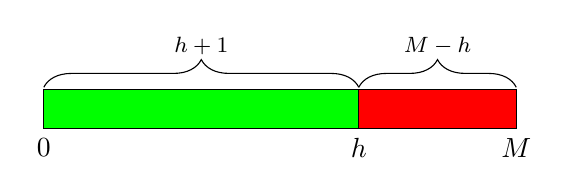
\begin{tikzpicture}
				\filldraw[fill=green, draw=black] (0,0) node[anchor=north] {$0$} -- (4,0) node[anchor=north] {$h$} -- (4,0.5) -- (0,0.5) -- (0,0);
				\filldraw[fill=red, draw=black] (4,0) -- (6,0) node[anchor=north] {$M$} -- (6,0.5) -- (4,0.5) -- (4,0);
				\draw [decorate,decoration={brace,amplitude=10pt},xshift=0pt,yshift=15pt]
				(0,0) -- (4,0) node [black,midway,yshift=15pt]{
					\footnotesize $h+1$
				};
				\draw [decorate,decoration={brace,amplitude=10pt},xshift=0pt,yshift=15pt]
				(4,0) -- (6,0) node [black,midway,yshift=15pt]{
					\footnotesize $M-h$
				};
			\end{tikzpicture}
			\end{center}
			Considering this, we could hit every integer below $h$ each with a probability of $1/(M+1)$, and we could hit exactly $h$ (since we're considering hits capped by $h$) with a probability of $(M-h)/(M+1)$. Averaging the expectations gives,
			\begin{align}
				\langle D \rangle_{h < M} &= \frac{1}{M+1}\sum_{i=0}^{h} i + \frac{M-h}{M+1}h \\
				&= \frac{1}{M+1}\frac{h(h+1)}{2} + \frac{M-h}{M+1}h \\
				&= \frac{h}{2}\frac{2M-h+1}{M+1}\\
				&= \frac{h}{2}\left(1 + \frac{M - h}{M+1}\right)\\
				&= \frac{h}{2}\left(2 - \frac{h + 1}{M+1}\right)
				% &= \frac{h^2}{2m} + \frac{h}{2m} + h - \frac{h^2}{m} \\
				% &= -\frac{h^2}{2m} + \left(\frac{1}{2m} + 1\right)h \\
			\end{align}

			Overall then, our expected damage on a successful hit is:
			\begin{align}
				\boxed{
					\langle D \rangle = \frac{1}{2}\begin{cases}
						M &\text{if $h \ge M$} \\
						h\left(2 - \frac{h + 1}{M+1}\right) &\text{if $h < M$} \\
					\end{cases}
				}
			\end{align}

			\begin{figure}
				\centering
				\includegraphics[width=\linewidth]{results/part_II/average_damage.pdf}
				\caption{The average damage of an attack with a maximum hit of $M$ on an opponent with $h$ health. The black line is the piecewise boundary.}
				\label{fig:average_d}
			\end{figure}


			This is plotted in Fig.~\ref{fig:average_d}. The Nukelawe model averages over these contributions for the \emph{overall} (i.e. not piecewise) expected hit, assuming each starting health is equally likely. This isn't totally accurate, regardless, it is good to check that our equations agree under this assumption:
			\begin{align}
				\langle D \rangle_\text{overall} &= \left \langle \langle D \rangle_{h < M} + \langle D\rangle_{h\ge M} \right \rangle\\
				&= \frac{1}{h_0}\left(\sum_{h<M} \langle D \rangle_{h < M} + \sum_{h\ge M}\langle D\rangle_{h\ge M} \rangle \right)\\
				&= \frac{1}{h_0}\left(
					\sum_{n=M+1}^{h_{0}}\frac{M}{2} +
					\sum_{n=1}^{y} \frac{n}{2}\left(2 - \frac{n + 1}{M+1}\right)
				\right) \\
				&= \frac{y(y+1)}{h_0(M+1)}\left(\frac{1}{2}{(M+h_0+1)}-\frac{1}{3}(2y+1) \right),
			\end{align}
			where $y=\min(M, h_0)$. The last step is actually quite tricky and involved to show. For that reason it can be found in Appendix~\ref{combat-app:power_reduction}. This agrees with Nukelawe's findings.

		\subsection{Health after \texorpdfstring{$n$}{} attacks}
			Despite the above being an ``average'', it is not the average damage expected per hit over the life time of an opponent since certain healths are much more likely to appear than others. As an example, suppose there is an opponent with 100 health fighting an attacker with a max hit of 30. On the first hit, the most likely health is 85. This means that unlike the above calculation, each hit is \emph{not} equally likely. Particularly, this over estimates the contribution in the overkill region, since (depending on the circumstances) let's say 1 or 2 hits is expected per kill. Those 1 or 2 hits are more likely to occur at specific $h$ values, but the average sums across all $h$ equally. In the non-overkill region, this has no impact due to it being constant. The proper treatment is to use the piecewise damage expectation in the recursive definition:
			\begin{align}
				h_{n+1} = h_{n} - \frac{1}{2}\begin{cases}
					M &\text{if $h_n \ge M$} \\
					h_n\left(2 - \frac{h_n + 1}{M+1}\right) &\text{if $h_n < M$}.
				\end{cases}
			\end{align}
			This however is too cumbersome to handle at once. Since the health is a decreasing monotonic function, we can consider it in two parts. While $h$ is above or equal to $M$ the solution to the above is the same as the Crude model's,
			\begin{align}
				h_n = h_0 - n\frac{M}{2}.\label{eq:h_crude}
			\end{align}
			The solution to the other is a bit more complex. After a certain number of iterations the health will drop below $M$ and the second case above will kick in. We'll say this occurs after $L$ iterations (noting that this \emph{average} quantity can be a non-integer),
			\begin{align}
				M &> h_0 - L\frac{M}{2} \\
				\frac{2}{M}(h_0 - M) &< L \\
				\implies L &= 2\left(\frac{h_0}{M} - 1\right).
			\end{align}
			Now the expected health that the second condition starts at is given by,
			\begin{align}
				\langle h_L \rangle &= h_0 - 2\left(\frac{h_0}{M} - 1\right) \frac{M}{2}\\
				&= M.
			\end{align}
			Thus the second case is expected to starts on iteration $L$ with an initial health of $M$. For simplicity, we will define $m\equiv n-L$. Returning to our recursive function,
			\begin{align}
				h_{m+1} &= h_{m} - \frac{h_m}{2}\left(2 - \frac{h_m + 1}{M+1}\right) \\
				&= h_{m} - h_m + \frac{h_m}{2}\frac{h_m + 1}{M+1} \\
				&= \frac{h_m^2 + h_m}{2(M+1)} \\
				h_{m+1} &= \gamma (h_m^2 + h_m), \label{eq:recur}
			\end{align}
			where $\gamma\equiv1 / 2(M+1)$. This type of recurrence relation is called a \href{http://mathworld.wolfram.com/QuadraticMap.html}{Quadratic Map}, and unfortunately it has no closed form solution in general. For the sake of completeness, we will call the solution to Eq.~\ref{eq:recur} $f(m; M, f_0)$. At this point we're left with,
			\begin{align}
					h(n; h_0, M) &=  \begin{cases}
					h_0 - \frac{1}{2}nM &\text{else if $n \le L$} \\
					f(n - L; M, M) &\text{otherwise}.
				\end{cases}
			\end{align}

			In general, we are more interested in the number of iterations that is required to kill an opponent which is the inverse of this function, $n=h^{-1}(h; h_0, M)$. However, since the recurrence relation cannot be solved analytically, we cannot obtain a general expression for this. We could numerically compute this result. However remember that we are dealing with \emph{expectation values} or averages. This means it is totally possible for the inverted function to say ``The opponents health will be 18 in 4.5 iterations, on average''. This is a problem because our recursive equation can only increment the iteration by one (and we can only start at $f_0$)! In the next section, we will look at an approximation that will allow us to handle non-integer expectations.

	\subsubsection{Approximate Solution}
			Despite not being able to find a closed-form solution for Eq.~\ref{eq:recur}, we can look for approximate solutions. Although it's rare, there are a few quadratic recurrence relations that \textbf{do} have solutions. There are two relevant cases, ones where a constant term is introduced, or ones where the linear term is removed. Since increasing $n$ (and therefore iterations) results in smaller and smaller $h_n$, it suggests that adding constant terms will heavily skew the results in this region. Removing the linear term is still not ideal since its contribution increases relative to the quadratic term, in the low $h_n$ limit (when this recursive case is required). However this should be less significant and we'll find that it does pretty well! If this justification does not satisfy you, please check out Appendix~\ref{combat-app:recursive_justification}. With this approximation, our recursive relation becomes,
			\begin{align}\label{eq:simplified_recursion}
				h_{m+1} = \gamma h_m^2.
			\end{align}
			Starting with $h_0 = M$, and looking at a few terms reveals,
			\begin{align}
				h_{1} &= \gamma^1 M^2\\
				h_{2} &= \gamma^1 h_1^2\\
					&= \gamma^1 \gamma^2 M^{(2\cdot2)}\\
				h_{3} &= \gamma^1 h_2^2\\
					&= \gamma^1 \gamma^2 \gamma^4 M^{(2\cdot2\cdot2)}\\
				\implies h_m &= \gamma^{\sum_{i=0}^{m-1} 2^i} M^{2^m}\\
							&= \gamma^{2^m-1} M^{2^m}\\
							&= \frac{1}{\gamma}(\gamma M)^{2^m}\\
						\Aboxed{h_m &= \frac{1}{\gamma}\left(\frac{1}{2} - \gamma\right)^{2^m}}
			\end{align}
			This equation is not only a closed form expression, but it can also be inverted!
			\begin{align}\label{eq:approximate_m}
				\log_2(\log_{\frac{1}{2} - \gamma} (\gamma h_m)) &= m.
			\end{align}
			This equation asymptotically reaches 0, but the opponent dying occurs when $h_m$ drops below 1 yielding an average kill on iteration,
			\begin{align}
				\log_2(\log_{\frac{1}{2} - \gamma} (\gamma)) &= m.
			\end{align}

			How can we make use of this approximation to improve our more accurate calculation? Remember that we are trying to solve the issue of non-integer iterations. Instead of beginning on iteration 0 for the iterative procedure, we can start $m$ at any real number in (0, 1), and iterate upwards on that. For example to get the health at iteration 4.87, we could use our analytic approximation to calculate 0.87 (which uses \textit{one} approximation), then iterate 4 times using the correct equation to get to the final result. So this defines our new best approximation,
			\begin{empheq}[box=\fbox]{align}\label{eq:recursive_h}
					h(n; h_0, M) &=  \begin{cases}
					h_0 - \frac{1}{2}nM &\text{if $n \le L$} \\
					\frac{1}{\gamma}\left(\frac{1}{2} - \gamma\right)^{2^{n-L}} &\text{if $n - L < 1$}\\
					f\left(n - L; M, \frac{1}{\gamma}\left(\frac{1}{2} - \gamma\right)^{2^{n-L}}\right) &\text{otherwise}\\
				\end{cases}\\
				\text{where, }\gamma = &\frac{1}{2(M+1)}\text{ and } L = 2\left(\frac{h_0}{M} - 1\right).\nonumber
			\end{empheq}

			\subsection{Attacks until \texorpdfstring{$h$}{} health}
				To solve for when the opponents health drops below one, $n=h^{-1}(1)$, we must use a numerical root finding algorithm to solve for the zero of $(1 - h(n))$. It is possible that $h^{-1}(1/2)$ is more representative of death than $h^{-1}(1)$. However, empirically, using 1 is in better agreement with simulation.

				The time complexity can be approximated using Eq.~\ref{eq:approximate_m}:
				\begin{align}
					\mathcal{O} &= \log_2(\log_{\frac{1}{2} - \gamma} (\gamma h_m))\\
					  &\propto \log\left( \frac{\log(\gamma h_m)}{\log (\frac{1}{2} - \gamma)}\right)\\
					  &\approx \log\left( \frac{\log(\frac{1}{\gamma h_m})}{\log (2)}\right)\\
					  &= \log\log\left(\frac{1}{\gamma h_m}\right) - \log\log (2)\\
					  &\sim \log\log\left(\frac{1}{\gamma h_m}\right)\\
					  &\approx \log\log\left(\frac{2m}{h_m}\right).
				\end{align}
				Here, $\propto$ is used to signal a multiplicative factor was ignored, and $\sim$ is used to signal an additive factor was ignored. In the first line the change of base formula was used, and the factor $log(2)$ was ignored. In the second line, $1/2-\gamma\approx1/2$ was used. This leaves us with $\mathcal{O}(\log\log(2m/h))$ evaluations required, which is practically constant. However, the number of evaluations for the numerical inversion depends on the implementation. In practice, at most 30 evaluations are required.


	\section{Approximately Analytic Recursion}
		\subsection{Health after \texorpdfstring{$n$}{} attacks}
			We can simplify the Recursive model by extending the approximation to all $n > L$:
			\begin{empheq}[box=\fbox]{align}
				h(n; h_0, M) &=  \begin{cases}
					h_0 - \frac{1}{2}nM &\text{if $n \le L$} \\
					\frac{1}{\gamma}\left(\frac{1}{2} - \gamma\right)^{2^{n-L}} &\text{otherwise}.
				\end{cases}
			\end{empheq}

		\subsection{Attacks until \texorpdfstring{$h$}{} health}
			This is useful because it can be inverted analytically:
			\begin{empheq}[box=\fbox]{align}
				n(h; h_0, M) &=  \begin{cases}
					(h_0 - h) \frac{2}{M} &\text{if $h \ge M$} \\
					\log_2(\log_{\frac{1}{2}-\gamma}(\gamma h)) &\text{otherwise}
				\end{cases}.
			\end{empheq}
			These can be evaluated in $\mathcal{O}(1)$ time.


	% \section{Markov Chain}

	\section{Health Regeneration}
		This is a method that considers health regeneration as piecewise averages. We start with one of our models which can give the health of the opponent after $n$ total attacks, $h(n; a, M, h_0)$ (without regeneration). Based on the weapon attack interval, $T_A$, we can convert to seconds through $t = nT_A$. This leaves us with $h(t/T_A; a, M, h_0)$. These equations cannot solve health regeneration since the health no longer decreases monotonically, and as a result the cases cannot be separated. Let's roll with this restriction and solve the problem within a window where the opponent does not heal. First we will make the assumption that the first regeneration occurs at $t=T_R$, which is the time between regenerations. We will later remove this restriction by averaging the first regeneration over $t\in[1, T_R]$. To reduce clutter, let's remove some explicit parameters and redefine $h$ as $h(t, h_0)$. The health just before the opponent heals is
		\begin{align}
			h_1 = h(T_R, h_{0}),
		\end{align}
		which is the health after $T_R$ seconds starting from some initial health $h_0$. Immediately after, the opponent will heal by $+1$ health,
		\begin{align}
			h_1 = h(T_R, h_{0}) + 1.
		\end{align}
		Iterating again:
		\begin{align}
			h_2 &= h(T_R, h_1) + 1 \\
				&= h(T_R, h(T_R, h_0) + 1) + 1.
		\end{align}
		Letting, $f(x)=h(T_R, x)$ to, again, reduce clutter and iterating again yields,
		\begin{align}
			h_3 &= f(h_2) + 1 \\
				&= f(f(h_1) + 1) + 1 \\
				&= f(f(f(h_0) + 1) + 1) + 1.
		\end{align}
		In general this gives us an \textit{iterated function},
		\begin{align}
			h_m &= g^{\circ m}(h_0),
		\end{align}
		where $m$ is the number of regeneration periods, and $g(x) \equiv f(x) + 1$. As an example of the function composition, for $m=2$ the above expands to:
		\begin{align}
			g^{\circ 2}(x)&=(g\circ g)(x)=g(g(x)) \\
						&=f(f(x) + 1) + 1.
		\end{align}
		This is great but this process doesn't continue indefinitely since the opponent will eventually die. There is a health, $h^*$ after which, the opponent will not be able to heal. Starting at a health of zero, we can determine how much health the player had $T_R$ seconds ago,
		\begin{align}
			h^* = h(-T_R, h_0=0)
		\end{align}
		Let's summarize. The opponent starts at $h_0$ health. They will not heal after $h^*$. The time taken to die is equal to the number of healing cycles until they drop below $h^*$. Plus the time it takes to get from that remaining health (not necessarily $h^*$) to 0. Pseudocode for this is given below, where \verb| health_after | and \verb| time_to_kill | are both non-regen functions. Parameters like accuracy and max hit are omitted.

		\begin{lstlisting}[language=Python, escapeinside={(*}{*)}]
def time_to_kill_regen(h_0):
h = (* $h_0$ *)
t = 0
(*$h^\ast$*) = health_after(-(*$T_R$*), 0)
while h (*$\ge$*) (*$h^\ast$*):
	h = health_after((*$T_R$*), h) + 1
	t += (*$T_R$*)
return t + time_to_kill(h)
\end{lstlisting}


		Now consider the initial condition. We assumed that the first regeneration occurred at $T_R$. However, it is a discrete (due to game ticks) uniform random variable distributed between $t_r \sim U[1, T_R]$. If a tick occurs every $\tau$ seconds, then there are $T_R/\tau$ game ticks before a heal.
		\begin{align}
			h_1 &= h(t_r, h_0) \\
			h_2 &= h(T_R, h(t_r, h_0) + 1) \\
			h_3 &= h(T_R, h(T_R, h(t_r, h_0) + 1) + 1) \\
			h_n &= (h\circ (x+1))^{\circ n-1}(T_R, h(t_r, h_0)) \\
			\langle h_n \rangle &= \frac{\tau}{T_R}\sum_{i=1}^{T_R/\tau} (h\circ (x+1))^{\circ n-1}(T_R, h(i\tau, h_0))
		\end{align}
		Now this has to be numerically inverted to give the time to kill.

	\section{Comparisons}
		We will only be comparing ``turns to \textit{kill}'' since ``turns to a given health'' is only possible with some models. In addition, since the health regeneration case adds additional complexities for expectedly minor improvements, it also won't be considered here.

		The combat is actually simple to simulate, however because it is a stochastic process that converges slowly getting high precision results is difficult this way. Regardless it can be done over the course of hours or days depending on the desired precision level. Our models can then be compared to these numerically simulated fights as is done in Fig.~(\ref{fig:comparison}). Regardless of the model, the turns to kill grows quickly when the max hit is low compared to the initial health of the opponent as shown in Fig.~\ref{fig:turns_to_kill}. By visual inspection, the time appears to scale roughly linearly with the health of the opponent, and exponentially with decreasing max hits.

		Looking closer at the graphs, the deviations between different models becomes more apparent. We can investigate this further by comparing the \textit{error} between the models' predictions and the simulation. Figure~\ref{fig:comparison} shows a wide variation in performance across these models. Most notably, the crude model performs the worst overall. Both the average and recursive methods have high error peaks, but otherwise do quite well. The Markov Chain model performs essentially perfectly, with it's approximation not falling far behind. Some statistics about the models are shown in Table~\ref{table:model_comp_stats}. Notably, the Markov Chain model has a significantly lower average error, standard deviation, and maximum error than all other models.

		\begin{table}[h]
		        \centering
		        \begin{tabular}{ l | c c c c }
		                Model & Average & Standard Deviation & Maximum & Minimum \\
		                \hline\hline
		                Crude & 18.14 & 18.54 & 98.20 & 1.75e-04 \\
		                Average & 10.29 & 17.92 & 73.00 & 8.85e-06 \\
		                MarkovChain & 0.06 & 0.06 & 0.62 & 7.35e-07 \\
		                MarkovChainApprox & 1.56 & 4.82 & 32.73 & 7.35e-07 \\
		        \end{tabular}
		        \caption{Error statistics for various models.}
		        \label{table:model_comp_stats}
		\end{table}

		Finally, one more interesting comparison to make is seeing which models perform best in which regions. Figure~\ref{fig:best_model} shows a heatmap depicting which models perform the best in which regions. There are several interesting trends that emerge (although their explanations are unknown but likely arbitrary). The comparison between all the models are done in three stages: first the crude, average, and recursive model are compared, then the Markov Chain Approximation is added, and finally all 5 models are compared. This is done since the Markov Chain models dominate, which would prevent us some seeing how the simpler models relate. The Crude model only makes an appearance when $M=1$ since overkill plays no role here and all models agree. The arbitrary ordering of evaluations places the Crude model first (but all models are equally valid here). In the first plot, we see that Average dominates the majority of the domain. However this is slightly mis-leading as the improvement over the Recursive model here is small, whereas in the region where the Recursive model dominates the improvement is substantial. Perhaps a better visualization would interpolate the colors depending on relative improvement. Regardless, in the next plot the Markov Chain Approximation quickly dominates essentially the whole domain. Finally, the last plot shows a battle between both Markov Chain models. However, there are a few details to note here. First there is a ``cut-out'' region at low max hits for which the Markov Chain model could not be evaluated due to numerical overflow in its current implementation. Second, it is strange that the approximation performs similarly well throughout and shares roughly equal domain (although this may be due to simply being such similar estimates). What makes this even more strange though is that a pattern emerges, in which the approximation seems to dominate at \textit{angles} in the domain i.e. lines with slopes that are multiples of $h_0/M$. There is no current explanation for this.
		\begin{figure}
			\centering
			\begin{subfigure}{0.5\linewidth}
				\centering
				\includegraphics[width=\linewidth]{results/part_II/turns_to_kill.pdf}
			\end{subfigure}%
			\begin{subfigure}{0.5\linewidth}
				\centering
				\includegraphics[width=\linewidth]{results/part_II/turns_to_kill_zoom.pdf}
			\end{subfigure}
			\caption{
				The number of successful turns to kill an opponent that has $h_0$ health, given that the attacker's max hit is $M$. The MarkovChain (hot colors) and Crude (cool colors) methods are shown. However, due to the scale of the left plot they are indistinguishable. The right plot shows a smaller region which allows for a comparison.
			}\label{fig:turns_to_kill}
		\end{figure}

		\begin{figure}
			\centering
			\includegraphics[width=\linewidth]{results/part_II/errors.pdf}
			\caption{
				A comparison between different models. The percent relative error with respect to the simulations are shown.
			}\label{fig:comparison}
		\end{figure}

		\begin{figure}
			\centering
			\includegraphics[width=\linewidth]{results/part_II/best_model.pdf}
			\caption{
				The model which agrees best with simulation, for different initial healths, and maximum hits. The final plot shows a comparison which includes all models. Since the MarkovChain (MC) models have very low errors, they occlude the other details. So, the other plots only include a subset of models. The leftmost only shows Crude, Average, and Recursive. The middle plot additionally includes MarkovChainApprox (MCApprox). Several interesting trends are discussed in the main body.
			}\label{fig:best_model}
		\end{figure}
		\chapter{Optimizing Player Equipment}
			In Section~\ref{sec:equipment_bonuses} we discussed the basic formulation of equipment bonuses. In this chapter, we will be interested in optimizing the player's choice of equipment to maximize some metric. Some examples of these metrics would be combat experience per hour, number of kills per hour, probability of winning, and so. Since the goal of the player may vary heavily, we aim to produce a general framework that can maximize arbitrary objective functions.

There are a large number of items that a player can equip in each slot, typically ranging from 10-100 considerations. Exhaustively considering each possible combination of equipment would result in roughly $10^{10}$ to $100^{10}$ possible sets. It is obvious then, that brute force would not work. We aim to reduce the number of possible equipments \textit{loadouts}, $\mathcal{L}$ that we must consider. A loadout is simply the set of equipment that a fighter is wearing:
\begin{align}
	\mathcal{L} = \{I_\text{slot}\,|\,\text{slot} \in \text{slots}\}.
\end{align}
To do this, we will reduce redundant equipment choices for each slot such that we end with a set of \emph{possibly} optimal loadouts. The only way to determine which of those is the actual optimal solution, $\mathcal{L}^*$ is to numerically evaluate the value of the objective, $f$, for each possibly optimal loadout. This defines our optimization problem as:
\begin{align}
	\mathcal{L}^* \leftarrow \mathop{\mathrm{argmin}}_{\mathcal{L} \in \{\mathcal{L}\}} f(\mathcal{L}).
\end{align}
So we will begin by reducing the size of the set $\{\mathcal{L}\}$.

\section{The Projection Vector}
	Different optimization problems require different information about the player's equipment. For example, when straightforwardly optimizing pure damage output (typically measured in kills per hour), the defensive bonuses of the player are irrelevant. By contrast, trying to maximize the probability of killing an opponent would require consideration of those defensive bonuses. Furthermore, a fighter only attacks with one attack style at a time. So clearly, not all bonuses are required for every optimization. For this reason, we introduce a \textit{projection} vector, $\vec{p}$, that will \emph{select} the bonuses that matter. Recall that our bonuses are divided into two groups: constant bonuses, and special bonuses. In Section~\ref{sec:equipment_bonuses}, we discussed how we treat special bonuses differently. So we will ignore them for now, and focus on the constant bonuses, $\vec{\mathcal{I}}_c^\text{slot}$. To select out the desired bonuses, we make $\vec{p}$ the same length as $\vec{\mathcal{I}}_c^\text{slot}$ so that each element in $\vec{p}$ corresponds to an equipment bonus. We can do so-called one-hot encoding, where we set elements to either 0 or 1 depending on whether the corresponding equipment bonus should be considered.

	An element-wise multiplication (also known as a Hadamard product) of these two vectors, $\vec{\mathcal{I}}_c^\text{slot} \odot \vec{p}$ contains the bonuses of the item that we want, and 0's for bonuses we don't want to consider. To compare different items we need to define a comparison operator, $\hat C (\cdot, \cdot)$ such that:
	\begin{align}
	    \hat C (\vec{\mathcal{I}}_{c, 1}^\text{slot}, \vec{\mathcal{I}}_{c, 2}^\text{slot}; \vec{p}) = \begin{cases}
	        1 \text{ if $\exists\,i\in [1, n]\,|\,(\vec{\mathcal{I}}_{c, 1}^\text{slot}  \odot \vec p)_i > (\vec{\mathcal{I}}_{c, 2}^\text{slot}  \odot \vec p)_i$} \\
	        0 \text{ otherwise},
	    \end{cases}
	\end{align}
	where $n$ is the number of bonuses for an item can have, and $(\cdot)_i$ represents the $i$'th bonus.
	By simply comparing the individual item bonuses, this term indicates whether some item, $\vec{\mathcal{I}}_{c, 1}^\text{slot}$, provides some advantage over another, $\vec{\mathcal{I}}_{c, 2}^\text{slot}$. If a given item doesn't provide some advantage over any other item then it doesn't need to be included in the set of equipment to consider. Note that $\hat C (\vec{\mathcal{I}}_{c, 1}^\text{slot}, \vec{\mathcal{I}}_{c, 1}^\text{slot}; \vec{p}) = 0$.

	\section{Set Reduction}
		With this, we can reduce the set of possible items in given slot, $\{\mathcal{I}^\text{slot}_j\}_{j=1}^{N_\text{slot}}$, where $N_\text{slot}$ is the number of possible items in that slot. We can define the following matrix,
		\begin{align}
		    \boldsymbol{A}^{\vec{p}} = A_{ij}^{\vec{p}} = \hat C (\vec{\mathcal{I}}_{c, i}^\text{slot}, \vec{\mathcal{I}}_{c, j}^\text{slot}; \vec{p}),
		\end{align}
		that is also one-hot encoded with 1's representing that the item in column $i$ provides some advantage over the item in row $j$, for our optimization problem.

		These individual item comparisons aren't too important, instead we care if an item may provide some advantage over \emph{any} other in the set. So, an item shouldn't be considered if the comparison yields 0 when compared against all other items:
		\begin{align}
		    &\sum_{i=1}^N \hat C (\vec{\mathcal{I}}_{c, j}^\text{slot}, \vec{\mathcal{I}}_{c, i}^\text{slot}; \vec{p}) = 0\\
		    \implies&\sum_{i=1}^N A_{ij}^{\vec{p}} = 0\\
		    \implies&\boldsymbol{1}\cdot\boldsymbol{A}_j^{\vec{p}} = 0
		\end{align}
		where $\boldsymbol{1}$ is a $N_\text{slot}$-dimensional vector containing ones, and $\boldsymbol{A}_j^{\vec{p}}$ is the $j$'th column in $\boldsymbol{A}^{\vec{p}}$.
		Then the reduced set of items for a given slot is then:
		\begin{align}
		    \{\mathcal{I}^\text{slot}_j; \vec{p}\}_{j=1}^{\bar{N}_\text{slot}} = \{\mathcal{I}_j^\text{slot}\,|\,\boldsymbol{1}\cdot\boldsymbol{A}_j^{\vec{p}} \neq 0,\,\,\, 1 \leq j \leq N_\text{slot}\},
		\end{align}
		where $\bar{N}_\text{slot}$ is the number of items left in this reduced set. The possibly optimal loadout set can be constructed as a ``$n$-ary'' Cartesian product:
		\begin{align}
			\{\bar{\mathcal{L}}; \vec{p}\} = \{(\mathcal{I}^\text{head}, ..., \mathcal{I}^\text{ring}) | \mathcal{I}^\text{slot} \in \{\mathcal{I}^\text{slot}_j; \vec{p}\}_{j=1}^{\bar{N}_\text{slot}} \,\forall\, \text{slot} \in \{\text{slots}\}\}
			% \{\mathcal{I}^\text{slot}_j; \vec{p}\}_{j=1}^{\bar{N}_\text{slot}}
		\end{align}
		% In future, it would be nice to see an example matrix for some arbitrary slot.

		As mentioned earlier, the choice of $\vec p$ depends on the problem at hand. However, only one attack style is generally considered and so often $\vec p$ can be chosen to only consider one attack style.\footnote{If the fighter switches weapons, or has multiple attacks, considering more than one attack style would then be required.} A natural formulation would be to iterate over each attack style. We can, for example, use $\vec{p}_\text{stab}$ to denote a projection vector which has stab as the only non-zero attack bonus. Then, the total set of considerations is the union of the specific attack style sets:
		% and disregarding weapons that cannot be used.
		\begin{align}
		    \{\bar{\mathcal{L}}; \vec{p}\} = \bigcup_{a\in \{\text{attack styles}\}}  \{\bar{\mathcal{L}}; \vec{p_a}\}.
		\end{align}
		This makes our optimization:
		\begin{align}
			\mathcal{L}^* \leftarrow \mathop{\mathrm{argmin}}_{\mathcal{L} \in \{\bar{\mathcal{L}}; \vec{p}\}} f(L),
		\end{align}
		which has reduced a search space containing billions of possibilities to one containing (empirically) less than 1,000.


		% (unless the fighter switches attack styles during the fight), only one
		\chapter{Optimizing Training Order}
			\section{Dijkstra's algorithm}
		
		\begin{appendices}
			\chapter{Justifying the Recursive Model Approximation}\label{app:analytic_form_attempt}
				We begin with Eq.~(\ref{eq:simplified_recursion}) which we will restate here with $h_m\to x_n$:
\begin{align}
	x_{n+1} = x_n - \frac{x_n}{2}\left(2 - \frac{x_n + 1}{M+1} \right).
\end{align}
This formulation looks similar to Newtons method for finding the root of $f(x)$, which is given as
\begin{align}
	x_{n+1} = x_n - \frac{f(x_n)}{f'(x_n)}.
\end{align}
After some algebra we find that,
\begin{align}
	\frac{f(x_n)}{f'(x_n)} = x_n(1-\gamma x_n).
\end{align}
This can be easily solved for $f(x)$ since this is a separable equation:
\begin{align}
	\frac{df}{f} &= \frac{dx}{x(1-\gamma x)} \\
	\int \frac{df}{f} &= \int \frac{dx}{x(1-\gamma x)} \\
	\ln(f) &= \ln|x| - \ln|\gamma x - 1| + C \\
	f(x) &= e^C |x||\gamma x - 1|
\end{align}
The error, $\epsilon$ in the next iteration of Newtons method is given as,
\begin{align}
	\epsilon_{n+1} = \epsilon_{n}^2 \left | \frac{f''(r)}{2f'(r)} \right |,
\end{align}
where $r$ is the root we desire. In this case the root we want is,
\begin{align}
	\lim_{n\to\infty} x_n = 0
\end{align}
since this corresponds to the health reaching zero. The ratio becomes,
\begin{align}
	\left| \frac{f''(r)}{2f'(r)} \right| = \gamma,
\end{align}
which simplifies the error equation to,
\begin{align}
	\epsilon_{n+1} = \gamma \epsilon_{n}^2.
\end{align}
This is exactly the same recursive equation we had before! Except that now we have error in health instead of health. So how does this connect? Since we already know the root value (which is 0), the error becomes the upper bound on the health. This means that if we have an error of, for example, 1 that the health must be below that. So, by solving $\epsilon=h$ we can find the number of iterations required to reach below that health. This solution is already given earlier but in the context of error we have,
\begin{align}
	\epsilon_{n} = \frac{1}{\gamma}\left( \frac{1}{2} - \gamma \right)^{2^{n}} \\
	n = \log_2 \log_{\frac{1}{2} - \gamma} (\gamma \epsilon).
\end{align}
This has done two things: justify the use exclusion of the $h_m$ term in the original recursive equation (instead of excluding $h^2_m$), and provided a second interpretation of the meaning of $h = 1$. The error comes from a Taylor series, but interestingly all higher order terms die off so this is actually exact. This suggests that for higher precision, the assumption that $\epsilon$ is small is violated and the Taylor series formulation no longer holds.

			\chapter{Power Reduction in the Piecewise Recursive Model}
				The average damage described in Section \ref{sec:average_damage} can be expanded to give,
\begin{align}
	\langle D \rangle_\text{overall} &= \frac{1}{h_0}\left(
		\sum_{n=M+1}^{h_{0}}\frac{M}{2} +
		\sum_{n=1}^{y} \frac{n}{2}\left(2 - \frac{n + 1}{M+1}\right)
	\right) \\
	&= \frac{1}{h_0}\left(
		\frac{M}{2}(h_0-y) +
		\sum_{n=1}^{y}n - \frac{1}{2}\sum_{n=1}^yn\frac{n + 1}{M+1}
	\right) \\
	&= \frac{1}{2h_0}\left(
		Mh_0-My + y(y+1)
		 - \frac{1}{2({M+1})}\sum_{n=1}^y(n^2 + n)
	\right) \\
	&= \frac{1}{2h_0}\left(
		Mh_0-My + y(y+1) - \frac{y(y+1)}{2({M+1})}
		 - \frac{y(n+1)(2y+1)}{6({M+1})}
	\right) \\
	&= \frac{1}{2h_0({M+1})}\left(
		M^{2}h_{0}-M^{2}y+My^{2}+yM+Mh_{0}-My - \frac{y^3-y}{3}
	\right) \\
	&= \frac{y(y+1)}{h_0({M+1})}\left(
		\frac{M(M+1)h_{0}}{2y(y+1)}+\frac{(y-M)M}{2(y+1)} - \frac{y-1}{6}
	\right) \\
	&= \frac{y(y+1)}{h_0({M+1})}\left(
		\frac{M(M+1)h_{0}}{2y(y+1)}+\frac{(y-M)M}{2(y+1)} +\frac{y+1}{2} -\frac{1}{3}(2y+1)
	\right)
	\label{eq:app-average-damage-original}
\end{align}
where $y=\min(M, h_0)$. In the second line, we used:
\begin{align}
	\sum_{a+1}^b1&=\begin{cases}
			b-a&\text{ if } b>a\\
			0 &\text{ else }
		\end{cases}\\
		&=b-\begin{cases}
			a &\text{ if } b>a\\
			0 &\text{ else }
		\end{cases}\\
		&=b-\min(a, b)
\end{align}
To finish, let's focus on,
\begin{align}
	 &\frac{M(M+1)h_{0}}{2y(y+1)}+\frac{(y-M)M}{2(y+1)} +\frac{y+1}{2} \\
	=&\frac{1}{2y(y+1)}\Big[ M(M+1)h_{0}+y(y-M)M +y(y+1)^2 \Big]\\
	=&\frac{1}{2y(y+1)}\Big[ M^2h_{0}+Mh_0+My^2-M^2y +y^3+2y^2+y \Big].\label{eq:app-average-damage-bracket}
\end{align}
This is a hard equation to simplify since the $M$'s and $h_0$'s are implicitly embedded in the $y$'s, but if you play with it long enough you can ``discover'' a way to simplify it - a form \textit{power reduction} that relies on getting rid of as many $y$'s as possible.

\section{Power Reduction}
	I'd like to preface the next part by saying the final result can easily be determined by plugging in $m$ as the $\min$, and $h_0$ as the $\min$ and combining the result. In this instance it works out nicely, but we will focus on general machinery to solve these problems assuming the solution was not so nice. Our goal here is to pull the $m$'s and $h_0$'s out of $y$. To do this, let's see if there is a way to construct $y^2$ from the other variables, specifically only using $y^1$. We know that if $M < h_0$, we need a term like $M^2$, and in the opposite case, we need a term like $h_0^2$,
	\begin{align}
		y^2 \sim M^2 \text{ or } h_0^2.
	\end{align}
	Based on this, we should be able to use $\min$ to switch between these two. So if we write the first term using $y$, we'd have something like $My$, which is true when $M$ is the minimum. If it isn't the minimum, there should be a second term which cancels the now $Mh_0$ term plus the required $h_0^2$ term:
	\begin{align}
		y^2 = My + h_0(y - M)\,\,\,\,\,(!)
	\end{align}
	Using the same logic, we can inductively deduce,
	\begin{align}
		\boxed{y^{n+1} = My^n + h_0^n(y - M) = My^n + h_0^ny - Mh_0^n.}
	\end{align}
	(and as an identity for the math people, with $\gamma = \min(a, b)$):
	\begin{align}
		\boxed{\gamma^{n+1} = a\gamma^n + b^n(\gamma - a) = a\gamma^n + b^n\gamma - ab^n}
	\end{align}
	In fact, this holds for $\max$ as well, or any \emph{similar} piece-wise function.
	Writing this as a recursive sequence by letting $g(n)=\gamma^n$ yields,
	\begin{align}
		g(n+1) = ag(n) + b^n(g(1) - a),
	\end{align}
	Under the initial condition $g(1)=\gamma$, \href{https://www.wolframalpha.com/input/?i=g%28n%2B1%29%3Da*g%28n%29%2Bb%5En%28C-a%29}{WolframAlpha} gives the general solution as,
	\begin{align}
		g(n) = a^n + (\gamma - a)\frac{a^n - b^n}{a - b} \\
		\boxed{g(n) = a^n + (\gamma - a)\sum_{i=0}^{n-1} a^{n-i-1}b^j,}
	\end{align}
	where the second line uses the difference of powers formula. This could have been solved by hand, but we've had enough fun with recursion in the other sections! This yields,
	\begin{align}
		g(1) &= \gamma\\
		g(2) &= a^2 + (\gamma - a)(a + b) \\
			&= a^2 + a\gamma - a^2  + b\gamma - ab \\
			&= a\gamma + b(\gamma - a) \\
		g(3) &= a^3 + (\gamma - a)\frac{a^3 - b^3}{a - b} \\
			&= a^3 + (\gamma - a)(a^2 + ab + b^2) \\
			&= a^3 + \gamma a^2 + \gamma ab + \gamma b^2 - a^3 - a^2b - ab^2 \\
			&= \gamma a^2 + \gamma ab + \gamma b^2 - a^2b - ab^2.
	\end{align}
	These agree with the original iterative equation. Okay, so this is a bit overkill since at most $y^3$ appears, so having general powers isn't too helpful. Nonetheless, we can now reduce the powers of $y$ in the original equation, and see how that simplifies things.
\section{Simplifying}
	We can now reduce the bracketed term in Eq.~\ref{eq:app-average-damage-bracket}:
	\begin{align}
	 	&\phantom{=}M^2h_0+Mh_0+My^2                   -M^2y + y^3                                    +2y^2+y \\
	 	&=M^{2}h_{0}+Mh_{0}+M^{2}y+h_{0}yM-h_{0}M^{2}-M^{2}y+yM^{2}+yMh_{0}+yh_{0}^{2}+\\
	 		&\phantom{=========} -M^{2}h_{0}-h_{0}^{2}M+2My+2h_{0}y-2h_{0}M+y\\
	 	&=\left(-M^{2}y+yM^{2}+M^{2}y+yMh_{0}+yh_{0}^{2}+2My+2h_{0}y+y+h_{0}yM\right)+\\
	 		&\phantom{=========} \left(M^{2}h_{0}+Mh_{0}-h_{0}M^{2}+-M^{2}h_{0}-h_{0}^{2}M-2h_{0}M\right)\\
	 	&=\left(2My+2h_{0}y+y+2yMh_{0}+M^{2}y+yh_{0}^{2}\right)+\left(-M^{2}h_{0}-h_{0}^{2}M-h_{0}M\right)
	\end{align}
	Having eliminated the ``hidden'' variables, let's try to re-group into powers of $y$:
	\begin{align}
	 	&=y^{2}+\left(My+h_{0}y+y+2yMh_{0}+M^{2}y+yh_{0}^{2}\right)+\left(-M^{2}h_{0}-h_{0}^{2}M\right)\\
	 	&=2y^{2}+y+2yMh_{0}+M^{2}y+yh_{0}^{2}+-M^{2}h_{0}-h_{0}^{2}M+Mh_{0}\\
	 	&=y^{2}M+y+y^{2}+y^{2}h_{0}+y^{2}+Mh_{0}\\
	 	&=y\left(yM+yh_{0}+y+M+h_{0}+1\right)\\
	 	&=y\left(y+1\right)\left(M+h_{0}+1\right)
	\end{align}
	Putting this into the corresponding term in Eq.~\ref{eq:app-average-damage-original} gives
	\begin{align}
		\frac{1}{2y(y+1)}y(y+1)\left(M+h_{0}+1\right) = \frac{1}{2}\left(M+h_{0}+1\right)
	\end{align}
	and so finally we arrive at,
	\begin{align}
		\boxed{\langle D \rangle_\text{overall} = \frac{y(y+1)}{h_0({M+1})}\left[
			 \frac{1}{2}\left(M+h_{0} + 1\right) -\frac{1}{3}(2y+1)
		\right]}.
	\end{align}
			\chapter{Fighting Probabilities}
				\section{Definitions}
\begin{align}
c_i & \text{ is the probability of doing $i$ damage} \\
c_0 & \text{ is the probability of doing zero damage} \\
c_+ &= 1 - c_0 \text{ is the probability of doing damage} \\
m & \text{ is the largest non-zero probability from $c_i$} \\
\end{align}

\section{Recursive Equation}
In one attack, the opponent can be brought to a given health $i$, from their initial health $h$ according to the transition probability, 
\begin{align}
	\pi_{h, i} &= \begin{cases}
		P(X=h - i) & \text{if } i > 0 \\
		P(X \ge h) & \text{if } i = 0
    \end{cases}
\end{align}
The probability they are killed in $L$ turns can be given by the sum of the probabilities the opponent was brought to $i$, then killed in $L - 1$ turns:
\begin{align}
	P_{h, L} &= \sum_{i=0}^\infty \pi_{h, i} P_{i, L-1}\\
	&= \cancel{\pi_{h, 0} P_{0, L-1}} + \pi_{h, h} P_{h, L-1} + \sum_{i=1}^{h-1} \pi_{h, i} P_{i, L-1} + \sum_{i=h+1}^\infty \pi_{h, i} P_{i, L-1}\\
	&= c_0P_{h, L-1} + \sum_{i=1}^{h-1} \pi_{h, i} P_{i, L-1} + \cancel{\sum_{i=h+1}^\infty \pi_{h, i} P_{i, L-1}}\\
	P_{h, L} &= c_0P_{h, L-1} + \sum_{i=\max(h-m, 1)}^{h-1} c_{h-i} P_{i, L-1}\\
\end{align}
where in the second line, the $i=0, h$ terms are explicitly considered, and the remaining sum is split in two. In the third line, $\pi_{h, i}$ would correspond to healing which we are taking to be zero. In the final line, we get the lower bound by considering that 
\begin{align}
	1\leq i \leq h-1 \implies& \pi_{h, i} = c_{h-i} \text{ if } 1\leq h - i \leq m \text{ otherwise } 0,\,\,\, \\
	\implies& 1\leq h - i \text{ and } h - i \leq m\\
	&\therefore  i\leq h - 1 \text{ and } h - m \leq i.
\end{align}
Since the first condition is already met, we have that $i \geq h - m$, but $i$ also cannot be below 1, hence $i\geq \max(h - m, 1)$. 



\section{Solution}
	The recursive equation to solve is:
	\begin{align}
		P_{h, L} &= c_0P_{h, L - 1} + \sum_{i\in I_h} c_{h-i} P_{i, L-1},\,\,\, L \ge 2, h \ge 1\\ % maybe 2
	\end{align}
	where $I_h$ is the set of integers satisfying $h - 1 \ge i \ge \max(h - m, 1)$. The boundary conditions are given by:
	\begin{align}
		P_{h, 1} &= \sum_{i=h}^m c_i \text{ (P of doing more than h damage)} \\
		 &= \theta(m - h) \sum_{i=h}^m c_i \\
		P_{1, L} &= c_+ c_0^{L-1} \text{ (P of missing $L-1$ times, then hitting any damage}\\
		P_{1, 1} &= c_+ \text{ (P of doing any damage)}
	\end{align}
	
	Using a generating function:
	\begin{align}
		g(x, y) &= \sum_{h=1}^\infty\sum_{L=1}^\infty P_{h, L} y^h x^L \\
		&= \sum_{h=1}^\infty\left(P_{h, 1} y^h x + \sum_{L=2}^\infty P_{h, L} y^h x^L \right)\\
		&= \sum_{h=1}^\infty P_{h, 1} y^h x + \sum_{h=1}^\infty\sum_{L=2}^\infty P_{h, L} y^h x^L\\
		&= xyP_{1, 1} + \sum_{h=2}^\infty P_{h, 1} y^h x + \sum_{L=2}^\infty\left( P_{1,L} yx^L + \sum_{h=2}^\infty P_{h, L} y^h x^L \right)\\
		&= xyP_{1, 1}  + x\sum_{h=2}^\infty P_{h, 1} y^h + \sum_{L=2}^\infty P_{1,L} yx^L + \sum_{L=2}^\infty\sum_{h=2}^\infty P_{h, L} y^h x \\
		&= xyP_{1, 1}  + x\sum_{h=2}^\infty P_{h, 1} y^h  + y\sum_{L=2}^\infty P_{1,L} x^L + \sum_{L=2}^\infty\sum_{h=2}^\infty P_{h, L} y^hx^L \\
	\end{align}
	These are the boundaries of a grid (corner $+$ top $+$ left) plus a sum over the interior. 

	\subsection{Corner} 
	Let's focus on each term at a time, starting with the corner:
	\begin{align}
		xyP_{1, 1} = xyc_+
	\end{align}
	\subsection{Top}
	For the top, lets first note that $\max(m - h + 1, 0)$ is non-zero when $m - h + 1 \ge 1 \implies m \ge h$. Then,
	\begin{align}
		x\sum_{h=2}^\infty P_{h, 1} y^h &= x \sum_{h=2}^\infty \theta(m - h)\sum_{i=h}^m c_i y^h\\
		&= x\sum_{h=2}^m \sum_{i=h}^m c_i y^h \\
	\end{align}
	\subsection{Left}
	Now the left:
	\begin{align}
		y\sum_{L=2}^\infty P_{1,L} x^L &= y\sum_{L=2}^\infty c_+ c_0^{L-1} x^L \\
		&= y\frac{c_+}{c_0}\sum_{L=2}^\infty (c_0x)^L \\
		&= y\frac{c_+}{c_0}\left[\sum_{L=0}^\infty (c_0x)^L - 1 - c_0x\right]\\
		&= y\frac{c_+}{c_0}\left[\frac{1}{1-c_0x} - 1 - c_0x\right]\\
		&= y\frac{c_+}{c_0}\frac{1}{1-c_0x}\left[1 - (1-c_0x) - (1-c_0x)c_0x\right]\\
		&= y\frac{c_+}{c_0}\frac{1}{1-c_0x}\left[c_0^2x^2\right]\\
		&= y\frac{c_+}{c_0}\frac{c_0^2x^2}{1-c_0x}\\
	\end{align}
	\subsection{Interior}
	Now the interior:
	\begin{align}
		\sum_{L=2}^\infty\sum_{h=2}^\infty P_{h, L} y^hx^L &= \sum_{L=2}^\infty\sum_{h=2}^\infty \left(c_0P_{h, L - 1} + \sum_{i\in I_h} c_{h-i}P_{i, L-1}\right) y^hx^L\\
		&= \sum_{L=2}^\infty\sum_{h=2}^\infty c_0P_{h, L - 1}y^hx^L + \sum_{L=2}^\infty\sum_{h=2}^\infty\sum_{i\in I_h} c_{h-i}P_{i, L-1}y^hx^L\\
		\mathcal{I}(x, y)&= G(x, y) + R(x, y).
	\end{align}
	Let us also tackle this individually, starting with the $G$ term:
	\begin{align}
		G(x, y) = \sum_{L=2}^\infty\sum_{h=2}^\infty c_0P_{h, L - 1}y^hx^L &= c_0\sum_{L=1}^\infty\sum_{h=2}^\infty P_{h, L}y^hx^{L+1}\\
		&= c_0x\sum_{L=1}^\infty\sum_{h=2}^\infty P_{h, L}y^hx^L\\
		&= c_0x\sum_{L=1}^\infty\left( \sum_{h=1}^\infty P_{h, L}y^hx^L -  P_{1, L}yx^L\right)\\
		&= c_0x\sum_{L=1}^\infty\sum_{h=1}^\infty P_{h, L}y^hx^L -  c_0xy\sum_{L=1}^\infty P_{1, L}x^L\\
		&= c_0xg(x, y) -  c_+ c_0xy\sum_{L=1}^\infty c_0^{L-1}x^L\\
		&= c_0xg(x, y) -  c_+ c_0x^2y\sum_{L=1}^\infty c_0^{L-1}x^{L-1}\\
		&= c_0xg(x, y) -  c_+ c_0 x^2y \sum_{L=0}^\infty c_0^{L}x^L\\
		&= c_0xg(x, y) -  \frac{c_+ c_0x^2y}{1-c_0x}\\
		&= c_0xg(x, y) -  y\frac{c_+}{c_0}\frac{c_0^2x^2}{1-c_0x}
	\end{align}
	
	% Followed by $R$. 
	% First let's note that $I$ is a non-empty set when $h-1>=\max(m-h, 1)$, empirically this is equivalent to:
	% $$h\ge \max\left(\left\lceil \frac{m + 1}{2} \right\rceil, 2\right)\equiv M \ge 2$$
	For $R$, we will first need a term that tells us whether $h$ is in the set $I$, i.e. does $h$ satisfy $h-1>=\max(m-h, 1)$? You will actually see that we need the more general $h-1>=\max(m-h+n, 1)$. We will call this condition $\delta_{m, h}^n$ which is $1$ if satisfied and $0$ otherwise. Empirically, this can be expressed as:
	\begin{align}
		\delta_{m, h}^n = \begin{cases}
			0 & \text{ if } h = 1 \\
			0 & \text{ if } n > m \\
			1 & \text{ otherwise } \\
		\end{cases}
	\end{align}
	Since $h >=2$,
	\begin{align}
		\delta_{m, h}^n = \delta_m^n = \begin{cases}
			1 & \text{ if } n \le m\\
			0 & \text{ otherwise } \\
		\end{cases}
	\end{align}
	Now solving $R(x, y)= \sum_{L=2}^\infty\sum_{h=2}^\infty\sum_{i\in I} c_{h-i}P_{i, L-1}y^hx^L$ gives:
	\begin{align}
		R(x, y) &= \sum_{L=2}^\infty\sum_{h=2}^\infty\sum_{i=\max(h-m, 1)}^{h-1} c_{h-i}P_{i, L-1}y^hx^L\\
		&= x \sum_{L=1}^\infty\sum_{h=2}^\infty\sum_{i=\max(h-m, 1)}^{h-1} c_{h-i}P_{i, L}y^hx^L\\
		&= xy \sum_{L=1}^\infty\sum_{h=1}^\infty\sum_{i=\max(h-m+1, 1)}^{h} c_{h-i}P_{i, L}y^hx^L\\
		&= xy \sum_{L=1}^\infty\sum_{h=1}^\infty\left(c_0P_{h, L}\delta_m^1 + \sum_{i=\max(h-m+1, 1)}^{h-1} c_{h-i}P_{i, L}\right)y^hx^L\\
		&= c_0xy \sum_{L=1}^\infty\sum_{h=1}^\infty P_{h, L}x^L\delta_m^1 + xy \sum_{L=1}^\infty\sum_{h=1}^\infty\sum_{i=\max(h-m+1, 1)}^{h-1} c_{h-i}P_{i, L}y^hx^L\\
	\end{align}
	Notice that the $h=1$ term in the second set of sums yields 0.
	\begin{align}
		&= c_0 xy g(x, y)\delta_h^1 + xy \sum_{L=1}^\infty\sum_{h=2}^\infty\sum_{i=\max(h-m+1, 1)}^{h-1} c_{h-i}P_{i, L}y^hx^L\\
		&= c_0xy g(x, y)\delta_h^1 + xy^2 \sum_{L=1}^\infty\sum_{h=1}^\infty\sum_{i=\max(h-m+2, 1)}^{h} c_{h-i}P_{i, L}y^hx^L\\
		&= c_0xy g(x, y)\delta_h^1 + xy^2 \sum_{L=1}^\infty\sum_{h=1}^\infty\left(\sum_{i=\max(h-m+2, 1)}^{h} c_{h-i}P_{i, L}\right)y^hx^L\\
		&= c_0xy g(x, y)\delta_h^1 + xy^2 \sum_{L=1}^\infty\sum_{h=1}^\infty\left(P_{i, L}\delta_m^2 + \sum_{i=\max(h-m+2, 1)}^{h} c_{h-i}P_{i, L}\right)y^hx^L\\
		&= c_0xy g(x, y)\delta_h^1 + xy^2 \sum_{L=1}^\infty\sum_{h=1}^\infty P_{i, L}\delta_m^2 + c_+xy^2 \sum_{L=1}^\infty\sum_{h=1}^\infty\sum_{i=\max(h-m+2, 1)}^{h} c_{h-i}P_{i, L}y^hx^L\\
		&= c_0xy g(x, y)\delta_h^1 + xy^2 g(x, y)\delta_m^2 + xy^2 \sum_{L=1}^\infty\sum_{h=1}^\infty\sum_{i=\max(h-m+2, 1)}^{h} c_{h-i} P_{i, L}y^hx^L\\
	\end{align}
	These series continues until the `engine' producing terms has no more. The number of terms in this series is given by the maximum $n$ that is non-zero:
	\begin{align}
		\arg \max_n \delta_m^n = m,
	\end{align}
	and so,
	\begin{align}
		R(x, y) &= c_+ x g(x, y)\sum_{i=1}^m y^i
	\end{align}
	% Followed by the recursive term (you'll see where it gets the name):
	% \begin{align}
	% 	c_+ \sum_{L=2}^\infty\sum_{h=2}^\infty\sum_{i\in I} P_{i, L-1}y^hx^L &= c_+ \sum_{L=1}^\infty\sum_{h=2}^\infty\sum_{i\in I_h} P_{i, L}y^hx^{L+1}\\
	% 	&= c_+ \sum_{h=2}^\infty\sum_{L=1}^\infty\sum_{i\in I_h} P_{i, L}y^hx^{L+1}\\
	% 	&= c_+ x\sum_{L=1}^\infty\sum_{h=2}^\infty\sum_{i\in I_h} P_{i, L}y^hx^L\\
	% 	&= c_+ x\sum_{L=1}^\infty x^L\left[\sum_{h=2}^\infty \sum_{i=\max(m-h, 1)}^{h-1} P_{i, L}y^h\right]\\
	% 	&= c_+ x\sum_{L=1}^\infty x^L\left[y\sum_{h=1}^\infty \sum_{i=\max(m-h-1, 1)}^{h} P_{i, L}y^h\right]\\
	% 	&= c_+ x\sum_{L=1}^\infty x^L\left[y\sum_{h=1}^\infty \left(P_{h, L}y^h + \sum_{i=\max(m-h-1, 1)}^{h-1} P_{i, L}y^h \right)\right]\\
	% 	&= c_+ x\sum_{L=1}^\infty x^L\left[y\sum_{h=1}^\infty P_{h, L}y^h + y\sum_{h=1}^\infty\sum_{i=\max(m-h-1, 1)}^{h-1} P_{i, L}y^h \right]\\
	% 	&= c_+ xy\sum_{L=1}^\infty \sum_{h=1}^\infty P_{h, L}y^hx^L + c_+ xy\sum_{L=1}^\infty x^L\sum_{h=1}^\infty\sum_{i=\max(m-h-1, 1)}^{h-1} P_{i, L}y^h \\
	% 	&= c_+ xyg(x, y) + c_+ xy\sum_{L=1}^\infty \sum_{h=1}^\infty\sum_{i=\max(m-h-1, 1)}^{h-1} P_{i, L}y^hx^L \\
	% 	&= c_+ xg(x, y) \left(y + y^2 + ...\right) \\
	% 	&= c_+ xg(x, y) \frac{1}{1-y} \\
	% \end{align}
	Now let's combine everything:
	\begin{align} 
		g(x, y) &= xyc_+ + x \sum_{h=2}^m \sum_{i=h}^{m}c_i y^h + \cancel{y\frac{c_+}{c_0}\frac{c_0^2x^2}{1-c_0x}} + c_0xg(x, y) - \cancel{y\frac{c_+}{c_0}\frac{c_0^2x^2}{1-c_0x}} +  x g(x, y)\sum_{i=1}^m c_{i} y^i\\
		&= x \sum_{h=1}^m\sum_{i=h}^{m}c_i y^h + c_0xg(x, y) + x g(x, y)\sum_{i=1}^m c_{i} y^i
	\end{align}
	Isolating for $g(x, y)$:
	\begin{align}
		g(x, y) - c_0xg(x, y) - x g(x, y)\sum_{i=1}^m c_{i} y^i &= x \sum_{h=1}^m\sum_{i=h}^{m}c_i y^h  \\
		g(x, y)\left[1 - c_0x - x \sum_{i=1}^m c_{i} y^i\right] &= x \sum_{h=1}^m\sum_{i=h}^{m}c_i y^h  \\
		g(x, y)\left[1 - x \sum_{i=0}^m c_{i} y^i\right] &= x \sum_{h=1}^m\sum_{i=h}^{m}c_i y^h  \\
		g(x, y) &= \frac{x \sum_{h=1}^m\sum_{i=h}^{m}c_i y^h}{1 - x \sum_{i=0}^m c_{i} y^i}
	\end{align}
	To simplify, let's define:
	\begin{align}
		T(y) &= \sum_{h=1}^m \sum_{i=h}^{m}c_i y^h\\
		B(y) &= \sum_{i=0}^m c_i y^i\\
	\end{align}
	Now $g(x, y)$ can be written as,
	\begin{align}
		g(x, y) &= T(y)\frac{x}{1- B(y)x}.
	\end{align}
	\newpage
	\subsection{Obtaining Power Series}
	%%%%%%%%%%%%%%%%%%%%%%%%%%%%%%%%%%%%%%%%%%%%%%%%%%%%%%%%%%%%%%%%
	To find the series representation of this, we will require the following identities:
	\begin{equation}\label{eq:binomial}
		(x + y)^n = \sum_{k=0}^n {n \choose k} x^{n-k}y^k
	\end{equation}
	\begin{equation}\label{eq:sub_binomial}
		(x - y)^n = \sum_{k=0}^n {n \choose k} (-1)^k x^{n-k}y^k
	\end{equation}
	\begin{equation}\label{eq:binomial_special}
		\frac{1}{(1-z)^\beta} = \sum_{k=0}^\infty {k + \beta -1 \choose k} z^k
	\end{equation}
	\begin{equation}\label{eq:geometric}
		\sum_{k=0}^n r^k = \frac{1 - r^{n+1}}{1 - r}
	\end{equation}
	%%%%%%%%%%%%%%%%%%%%%%%%%%%%%%%%%%%%%%%%%%%%%%%%%%%%%%%%%%%%%%%%

	Let us start with:
	\begin{align}
		\frac{1}{1- B(y)x} &= \sum_{k=0}^\infty B^k(y)x^k \\
	\end{align}
	We need to workout $B^k(y)$:
	\begin{align}
		B^k(y) &= \left( \sum_{j=0}^m c_j y^j\right)^k \\
		&= \sum_{j=0}^{km} d_j^k y^j,
	\end{align}
	where $d_j^k$ is the $j$'th element of the $k$'th convolution of $c$, which doesn't have an analytic form. In practice the \texttt{numpy} function \texttt{numpy.polynomial.polynomial.polypow} can be used to compute this. Then,
	% https://en.wikipedia.org/wiki/Discrete_Fourier_transform#Polynomial_multiplication
	% https://caps.gsfc.nasa.gov/simpson/pubs/series.pdf also
	\begin{align}
		\frac{1}{1-B(y)x} &= \sum_{k=0}^\infty \left[ \sum_{j=0}^{km} d_j^k y^j \right] x^k \\
		\implies\frac{x}{1-B(y)x} &= \sum_{k=0}^\infty \left[ \sum_{j=0}^{km} d_j^k y^j \right] x^{k+1} \\
		&= \sum_{k=1}^\infty \sum_{j=0}^{(k-1)m} d_j^{k-1} y^j x^k
	\end{align}

	Multiplying by $T(y)$ gives back our generating function:
	\begin{align}
		g(x, y) = \frac{T(y)x}{1-B(y)x} &= T(y)\sum_{k=1}^\infty \sum_{j=0}^{(k-1)m} d_j^{k-1} y^j x^k\\
		&= \sum_{h=1}^m \sum_{i=h}^{m}c_i y^h \cdot \sum_{k=1}^\infty \sum_{j=0}^{(k-1)m} d_j^{k-1} y^j x^k\\
		&= \sum_{h=1}^m  \sum_{k=1}^\infty \sum_{j=0}^{(k-1)m} \sum_{i=h}^{m} c_i d_j^{k-1} y^{j+h} x^k\\
		&= \sum_{h=1}^m  \sum_{k=1}^\infty \sum_{j=0}^{(k-1)m} a_{h, j}^k y^{j+h} x^k,
	\end{align}
	where $a_{h, j}^k \equiv \sum_{i=h}^{m} c_i d_j^{k-1}$. We make use of the identity (visual proof omitted)
	\begin{align}
		\sum_{i=1}^N \sum_{j=0}^M a_{i, j}y^{i+j} = \sum_{p=1}^{N+M}\left[ \sum_{j=\max(1, p-M)}^{\min(p, N)} a_{j, p-j}\right]y^p
	\end{align}
	with $h=i, j=j, N=m, M=(k-1)m$ to obtain:
	\begin{align}
		g(x, y) &= \sum_{k=1}^\infty \sum_{p=1}^{km} \left[\sum_{j=\max(1, p+(1-k)m)}^{\min(p, m)} a_{j, p-j}^k \right]y^px^k\\
		 &= \sum_{L=1}^\infty \sum_{h=1}^{Lm} \left[\sum_{j=\max(1, h+(1-L)m)}^{\min(h, m)} a_{j, h-j}^L \right]y^h x^L\\
		 &= \sum_{L=1}^\infty \sum_{h=1}^{\infty} \left[\theta(Lm-h)\sum_{j=\max(1, h+(1-L)m)}^{\min(h, m)} a_{j, h-j}^L \right]y^h x^L
	\end{align}
	where $\theta(x)$ is the Heaviside function. Extracting out $P_{h, L}$, we get,
	\begin{align}
		P_{h, L} &= \theta(Lm-h)\sum_{j=\max(1, h+m-mL)}^{\min(h, m)} a_{j, h-j}^L \\
		P_{h, L} &= \theta(Lm-h)\sum_{j=\max(1, h+m-mL)}^{\min(h, m)} \sum_{i=h}^m c_i d_{h-j}^{L-1}
	\end{align}
	And so we end with:
	\begin{equation}
		\boxed{\therefore P_{h, L} = \theta(Lm-h)\sum_{j=\max(1, h+m-mL)}^{\min(h, m)} \sum_{i=h}^m c_i d_{h-j}^{L-1} }
	\end{equation}
	

	\section{Summing over $L$}
		Often, the following quantity needs to be evaluated for further applications, like the probability of winning a fight:
		\begin{equation}
			\sum_{L=b}^\infty P_{h, L} = P_{h, 1}\sum_{L=b}^\infty c_0^{L-1}  + \sum_{i=1}^{\min(h, m)} \sum_{L=b}^\infty H_{h, i}^L,
		\end{equation}
		

		Tackling the first term, we get: % https://en.wikipedia.org/wiki/Geometric_progression, related formulas
		\begin{align}
			\sum_{L=b}^\infty c_0^{L-1} &= \sum_{L=b-1}^\infty c_0^{L} \\
			&= \frac{c_0^{b-1}}{1 - c_0} \\
		\end{align}

		% \newpage
		For the second term, we need:
		\begin{align}
			\sum_{i=a}^\infty {i \choose k} x^i &= \sum_{i=1}^\infty {i \choose k} x^i - \sum_{i=1}^{a-1} {i \choose k} x^i,\,\,\,1\leq k \leq a\\
			&= \frac{x^k}{(1-x)^{k+1}} - \sum_{i=1}^{a-1} {i \choose k} x^i\\
		\end{align}

		Focusing on the second term,
		\begin{align}
			\sum_{L=b}^\infty H_{h, i}^L &= C_i \sum_{L=b}^\infty  c_0^{L-1} \sum_{p=1}^{\min_{h-i}^{L-1}} {L-1 \choose p}  G(h, i, p)\\
			&= C_i \sum_{L=b}^\infty  \left[ \sum_{p=1}^{\min_{h-i}^{L-1}} c_0^{L-1}{L-1 \choose p}  G(h, i, p) \right]\\
			&= C_i \sum_{L=b}^{h-i} \sum_{p=1}^{L-1} c_0^{L-1}{L-1 \choose p}  G(h, i, p) + C_i \sum_{L=\max^b_{h-i+1}}^{\infty} \sum_{p=1}^{h-i} c_0^{L-1}{L-1 \choose p}  G(h, i, p)\\
			&= C_i \sum_{L=b}^{h-i} \sum_{p=1}^{L-1} c_0^{L-1}{L-1 \choose p}  G(h, i, p) + C_i  \sum_{p=1}^{h-i} \left[\sum_{L=\max^b_{h-i+1}}^{\infty} c_0^{L-1}{L-1 \choose p}  \right]G(h, i, p)\\
			&= C_i \sum_{L=b}^{h-i} \sum_{p=1}^{L-1} c_0^{L-1}{L-1 \choose p}  G(h, i, p) + C_i  \sum_{p=1}^{h-i} \left[\sum_{L=\max^{b-1}_{h-i}}^{\infty} c_0^{L}{L \choose p}  \right]G(h, i, p)\\
			&= C_i \sum_{L=b}^{h-i} \sum_{p=1}^{L-1} c_0^{L-1}{L-1 \choose p}  G(h, i, p) + C_i  \sum_{p=1}^{h-i} \left[\sum_{L=0}^{\infty} c_0^{L}{L \choose p} - \sum_{L=0}^{\max^{b - 1}_{h - i} - 1} c_0^{L}{L \choose p}  \right]G(h, i, p)\\
			&= C_i \sum_{L=b}^{h-i} \sum_{p=1}^{L-1} c_0^{L-1}{L-1 \choose p}  G(h, i, p) + C_i  \sum_{p=1}^{h-i} \left[\frac{c_0^p}{(1-c_0)^{p+1}} - \sum_{L=0}^{\max^{b - 1}_{h - i} - 1} c_0^{L}{L \choose p}  \right]G(h, i, p)\\
			&= C_i \sum_{L=b}^{h-i} \sum_{p=1}^{L-1} c_0^{L-1}{L-1 \choose p}  G(h, i, p) + C_i  \sum_{p=1}^{h-i} \left[\frac{c_0^p}{(1-c_0)^{p+1}} - \sum_{L=1}^{\max^{b - 1}_{h - i} - 1} {L \choose p} c_0^L \right]G(h, i, p)  % Since j=0 term is zero.
		\end{align}
		Having removed any infinities, this equation is now computationally feasible. It can be used in further calculations like the probability a player kills their opponent before they are killed.









	% If we define,
	% \begin{align}
	% 	A_{j, k} \equiv \sum_{i=0}^{\min(\lfloor j / m \rfloor, k)} a_{i, j-mi}^k,
	% \end{align}
	% then,
	% \begin{equation}
	% 	\sum_{j=0}^\infty \sum_{i=0}^k a_{i, j}^k y^{mi +j} = \sum_{j=0}^\infty A_{j, k}y^j.
	% \end{equation}
	% and so,
	% \begin{align}
	% \sum_{k=1}^\infty \left[ \sum_{j=0}^\infty \sum_{i=0}^k a_{i, j}^k y^{mi +j}\right]y^k x^k &= \sum_{k=1}^\infty \left[\sum_{j=0}^\infty A_{j, k}y^j \right] y^kx^k\\
	% &= \sum_{k=1}^\infty \sum_{j=0}^\infty A_{j, k} y^{k+j}x^k\\
	% &= \sum_{k=1}^\infty \sum_{n=k}^\infty A_{n-k, k} y^{n}x^k\\
	% \end{align}
	% Therefore,
	% \begin{align}
	% \frac{1}{1-B(y)x} &= 1 + \sum_{k=1}^\infty \sum_{n=k}^\infty A_{n-k, k} y^{n}x^k\\
	% \implies\frac{x}{1-B(y)x} &= x + \sum_{k=1}^\infty \sum_{n=k}^\infty A_{n-k, k} y^{n}x^{k+1}\\
	% &= x + \sum_{k=2}^\infty \sum_{n=k-1}^\infty A_{n-k+1, k-1} y^{n}x^k\\
	% \end{align}
	% Now,
	% \begin{align}
	% T(y)\frac{x}{1-B(y)x} &= T(y)x + T(y)\sum_{k=2}^\infty \sum_{n=k-1}^\infty A_{n-k+1, k-1} y^{n}x^k\\
	% &= T(y)x + c_+ \sum_{h=1}^m (m - h + 1)y^h\sum_{k=2}^\infty \sum_{n=k-1}^\infty A_{n-k+1, k-1} y^{n}x^k\\
	% &= T(y)x + c_+ \sum_{k=2}^\infty \sum_{n=k-1}^\infty \left[\sum_{h=1}^m (m - h + 1)A_{n-k+1, k-1} y^{n+h} \right]x^k\\
	% \end{align}
	% Define,
	% \begin{align}
	% 	\gamma_{n, k}^h \equiv (m - h + 1)A_{n-k+1, k-1}
	% \end{align}
	% Now,
	% \begin{align}
	% 	T(y)\frac{x}{1-B(y)x} &= T(y)x + c_+ \sum_{k=2}^\infty \left[\sum_{n=k-1}^\infty \sum_{h=1}^m \gamma_{n, k}^h y^{h+n} \right]x^k\\
	% \end{align}
	% To handle this, we make use of the identity [visual proof is also omitted]:
	% \begin{align}
	% 	\sum_{n=b}^\infty \sum_{h=1}^m a_{n, h} y^{n+h} = \sum_{n=b+1}^\infty\left( \sum_{h=1}^{\min(n-b, m)}a_{n-h, h} \right) y^n
	% \end{align}
	% So now,
	% \begin{align}
	% 	g(x, y) &= T(y)x + c_+ \sum_{k=2}^\infty \left[\sum_{n=k}^\infty\left( \sum_{h=1}^{\min(n-k+1, m)}\gamma_{n-h, k}^h \right) y^n \right]x^k\\
	% 	&= T(y)x + \sum_{k=2}^\infty \sum_{n=k}^\infty\left( \sum_{h=1}^{\min(n-k+1, m)}c_+\gamma_{n-h, k}^h \right) y^n x^k\\
	% \end{align}
	% With a change of variables we get,
	% \begin{align}
	% 	\sum_{L=1}^\infty \sum_{h=1}^\infty P_{h, L} y^h x^L &= T(y)x + \sum_{L=2}^\infty \sum_{h=L}^\infty\left( \sum_{i=1}^{\min(h-L+1, m)}c_+\gamma_{h-i, L}^i \right) y^h x^L\\
	% 	\sum_{h=1}^\infty P_{h, 1} y^h x + \sum_{L=2}^\infty \sum_{h=1}^\infty P_{h, L} y^h x^L &= T(y)x + \sum_{L=2}^\infty \sum_{h=L}^\infty\left( \sum_{i=1}^{\min(h-L+1, m)}c_+\gamma_{h-i, L}^i \right) y^h x^L\\
	% 	% \implies P_{h, L} &= c_+ \sum_{j=1}^{\min(h - L + 1, m)} \gamma_{h-j, L}^j\\
	% \end{align}
	% Since the $x$ terms are trivially a boundary condition, let's focus on the double sums:
	% \begin{align}
	% 	\sum_{L=2}^\infty \sum_{h=1}^\infty P_{h, L} y^h x^L &= \sum_{L=2}^\infty \sum_{h=L}^\infty D_{h, L} y^h x^L\\
	% 	% \implies P_{h, L} &= c_+ \sum_{j=1}^{\min(h - L + 1, m)} \gamma_{h-j, L}^j\\
	% \end{align}
	\newpage
	\section{Summary}
		First, given a player's max hit of $m$ and an opponent's initial health of $h$, we define:
		\begin{align}
			c_+ &= \frac{a}{m+1} \\
			c_* &= mc_+ \\
			c_0 &= 1 - c_* \\
			C_i &= c_+ (m - i + 1)
		\end{align}
		where $c_0$ is the probability of doing zero damage, and $c_+$ is the probability of doing any positive amount of damage.
		Then, the probability of killing in $L$ turns is given by the recursive equation:
		\begin{align}
			P_{h, L} &= c_0P_{h, L - 1} + c_+ \sum_{i=\max{h - m, 1}}^{h-1} P_{i, L-1},\,\,\, L \ge 2, h \ge 1
		\end{align}
		The boundary conditions are given by:
		\begin{align}
			P_{h, 1} &= c_+ \max(m - h + 1, 0)\\
			P_{1, L} &= c_* c_0^{L-1}\\
			P_{1, 1} &= c_*
		\end{align}
		This has the following solution:
		\begin{equation}
			P_{h, L} = P_{h, 1}c_0^{L-1}  + \sum_{i=1}^{\min(h, m)} H_{h, i}^L,
		\end{equation}
		where
		\begin{align}
			H_{h, i}^L &\equiv c_+c_0^{L-1} (m - i + 1)\sum_{p=1}^{\min_{h-i}^{L-1}} {L-1 \choose p}  G(h, i, p) \\
			G(h, i, p) &\equiv \left(\frac{c_+}{c_0}\right)^p  \sum_{l=0}^{\min_{\lfloor (h-i-p) / m \rfloor}^{p}} (-1)^l  {p \choose l} {h-i-ml-1\choose h-i-ml-p}.
		\end{align}
		The probability of winning a fight with an opponent, and drawing is given by:
		\begin{align}
			P_\text{win} &= \sum_{L=1}^\infty \sum_{l=L+1}^\infty P_{h_\text{player}, l}^{m_\text{opponent}} P_{h_\text{opponent}, L}^{m_\text{player}}\\
			P_\text{draw} &= \sum_{L=1}^\infty P_{h_\text{player}, L}^{m_\text{opponent}} P_{h_\text{opponent}, L}^{m_\text{player}},
		\end{align}
		where $P_\text{win} + P_\text{lose} + P_\text{draw} = 1$ and swapping opponent values for player values turns $P_\text{win}$ into $P_\text{lose}$. The sum $\sum_{L=a}^\infty P_{h, L}$ can also be expressed in terms of a finite sum.

	\section{Comments}
		It would be useful to compute the time complexity required for evaluation. There is an infinite sum in both $P_\text{win}$ and $P_\text{lose}$ that must simply be truncated during evaluation. It would be nice to either find analytic solutions or determine appropriate cutoffs.
	

		\end{appendices}

	\part{Woodcutting}
	\part{Mining}
	\part{Quests}

\bibliographystyle{unsrt}
\bibliography{main}

\end{document}